%% What Right-Angle Corners Reveal About an Uncalibrated Camera
%% Springer Nature journal template (sn-jnl, December 2024), Math and Physical Sciences numbered reference style.
%% Two-column layout (iicol), as the journal recommends; remove iicol for a single-column draft.
\documentclass[pdflatex,sn-mathphys-num,iicol]{sn-jnl}

\usepackage[T1]{fontenc}
\input{glyphtounicode}\pdfgentounicode=1
\usepackage[utf8]{inputenc}
\usepackage{lmodern}
\usepackage{microtype}
\usepackage{amsmath,amssymb,amsfonts}
\usepackage{bm}
\usepackage{graphicx}
\usepackage{booktabs,tabularx,array}
\usepackage{xcolor}
\usepackage{tikz}
\usetikzlibrary{arrows.meta,calc}
\usepackage{xurl}% lets long URLs in the references break across lines
\def\burl#1{\url{#1}}% the reference style's URL command, made breakable
\usepackage[capitalise,noabbrev]{cleveref}

% ---------------------------------------------------------------- macros
\newcommand{\vd}{\mathbf{d}}
\newcommand{\vr}{\mathbf{r}}
\newcommand{\vt}{\mathbf{t}}
\newcommand{\vn}{\mathbf{n}}
\newcommand{\vl}{\mathbf{l}}
\newcommand{\vc}{\mathbf{c}}
\newcommand{\vw}{\mathbf{w}}
\newcommand{\vg}{\mathbf{g}}
\newcommand{\vv}{\mathbf{v}}
\newcommand{\fmin}{f_{\min}}
\newcommand{\vh}{\mathbf{h}}
\newcommand{\vm}{\mathbf{m}}
\newcommand{\OR}{Online Resource~1}
\newcommand{\TODO}[1]{\textcolor{red}{[TODO: #1]}}


\theoremstyle{thmstyleone}
\newtheorem{theorem}{Theorem}
\newtheorem{proposition}[theorem]{Proposition}
\newtheorem{lemma}[theorem]{Lemma}
\newtheorem{corollary}[theorem]{Corollary}
\theoremstyle{thmstylethree}
\newtheorem{definition}[theorem]{Definition}
\theoremstyle{thmstyletwo}
\newtheorem{remark}[theorem]{Remark}

\raggedbottom

\begin{document}

\title[What Right-Angle Corners Reveal About an Uncalibrated Camera]{What Right-Angle Corners Reveal About an Uncalibrated Camera: Convex Cones, Certified Bounds and Identifiability}

\author*{\fnm{Michael} \sur{Werman}}\email{michael.werman@mail.huji.ac.il}

\affil{\orgdiv{School of Computer Science and Engineering}, \orgname{The Hebrew University of Jerusalem}, \orgaddress{\city{Jerusalem}, \country{Israel}}}

\abstract{The corner of a box or a room, where three perpendicular edges meet, appears in an image as three segments meeting at a point. We ask what such junctions reveal about an uncalibrated camera's intrinsic parameters. Each junction is consistent with an explicit convex set of cameras; when only the focal length is unknown, this set is an interval in closed form. These sets are computed from the image alone, so calibrating from many junctions is a convex feasibility problem. Almost every junction bounds the focal length from below; we characterize when one also bounds it from above, and when many junctions determine it exactly. For a known vertex, the bounds can be certified against any bounded error in the measured edge directions.}

\keywords{camera calibration, absolute conic, right-angle corners, Manhattan world, identifiability, convex feasibility\\[4pt]\textbf{MSC Classification:} 68T45, 68U10, 65D19, 51N15, 52A20, 90C25}

\maketitle

% ======================================================================
\section{Introduction}\label{sec:intro}

A right-angle corner, three mutually perpendicular edges meeting at a point, appears in an image as a junction of three line segments. Such corners are ubiquitous: on boxes, in rooms, at doorframes and on furniture. Unlike a generic feature point, a corner carries metric information, namely three directions known to be mutually orthogonal. This paper asks what such junctions reveal about the intrinsic parameters of the camera that images them. The contribution is theoretical: without locating any vanishing point, we determine exactly which cameras junctions can rule out, each by a single junction, and which no junction can exclude. The answer gives bounds on the camera that the data guarantee, even when there are too few lines to find vanishing points.

Earlier work on what a camera learns from right-angle corners covers two extremes: a single corner seen by a calibrated camera, and a whole box seen by an uncalibrated one. For a single junction and a calibrated camera, \citet{perkins1968} and \citet{kanade1980} analyzed orthographic images of trihedral corners, and \citet{barnard1983} and \citet{horaud1987} back-projected the image lines to interpretation planes. \citet{kanatani1986} derived the closed form under orthography, with its two junction types, fork and arrow. \citet{kanatani1988} and \citet{shakunaga1986,shakunaga1989} extended the analysis to perspective: the orientation is unique up to a mirror, and a condition decides whether a junction can be the image of a right-angle corner at all. The closest precedent for reading that condition as a feasibility problem is the labeling of line drawings \citep{huffman1971,clowes1971}, in particular the algebraic treatment of \citet{sugihara1986}, which decides whether a drawing is realizable by solving a linear feasibility problem. At the other extreme, for a whole parallelepiped and an uncalibrated camera, \citet{wilczkowiak2001,wilczkowiak2002,wilczkowiak2005} fit a canonic projection matrix to six or more vertices; each right angle then contributes one linear equation on the calibration.

The common case lies between these extremes: an uncalibrated camera that sees one corner or a few, as in an image of a room or of a single object. Existing methods treat such scenes by exploiting long line families: Manhattan-world methods \citep{coughlan1999,schindler2004}, calibration from vanishing points \citep{caprile1990,cipolla1999,kosecka2002,wildenauer2012}, single-view metrology \citep{criminisi2000} and vanishing-point detection \citep{tardif2009}. Other approaches require more structure: \citet{jelinek2001} need a full polyhedral model with model-to-image correspondences, and \citet{ramalingam2013} combine Manhattan junctions with vanishing points to estimate indoor layout, as do the layout methods of \citet{hedau2009} and \citet{lee2009}. Learned calibrators \citep{workman2015,holdgeoffroy2018,jin2023,veicht2024} regress the camera directly from pixels. We ask instead what the individual junctions determine.

The starting point is a simple observation. Each image line of a junction back-projects to a plane through the camera center, and because the three lines meet at the image of the vertex, all three planes contain the same viewing ray. For every calibration matrix $K$, this turns the condition that the junction be the image of a right-angle corner into the negativity of a product of three forms, each linear in the dual image of the absolute conic $\omega^{*}=KK^{\top}$ (\cref{prop:general}). In plain terms, the cameras for which a junction can be the image of a right-angle corner form a region bounded by three planes in the space of cameras. Among positive-definite forms this region is a convex cone, the positive combinations of three rank-one forms on the plane of lines through the junction (\cref{thm:convex}); when only the focal length is unknown, the cone reduces to an interval with closed-form endpoints (\cref{thm:interval}). Since each junction's constraint is computed from the image alone, calibration from junctions is a convex feasibility problem (\cref{sec:program}).

Junctions become far more informative when several corners belong to one rectilinear structure, such as a building or a room, whose edges all run along the same three perpendicular directions, a Manhattan frame. The edges of all its corners then converge on the same three vanishing points. Call the line through two of these vanishing points the \emph{edge-on line} of the third direction; classically, it is the vanishing line of the planes perpendicular to that direction. The name records what happens to a corner whose vertex lies on this line: the face spanned by its other two edges is seen edge-on, and those two edges appear as a single image line. These lines organize the main result.
Each junction still imposes only an inequality, but together the junctions of one frame decide exactly which cameras can be rejected (\cref{thm:converse}). When the edge-on line of a direction \emph{passes through} the image, meeting it in a segment (\cref{fig:vlines}), every camera under which that direction's vanishing point is not orthogonal to the other two is rejected by some junction near that line. Conversely, cameras that satisfy these orthogonalities and lie near the true one pass every junction, so no set of junctions can reject them. Junctions therefore never carry more information than the vanishing points, and strictly less when fewer than two edge-on lines pass through the image. We say that junctions \emph{determine} a parameter when every wrong value is rejected by some junction.

Three consequences follow. For the focal length alone, one frame determines it when the edge-on line of a direction tilted out of the image plane passes through the image (\cref{thm:identframe}), and a junction bounds it from above exactly when its vertex lies in a region bounded by circles whose diameters join pairs of vanishing points (\cref{thm:boundmap}). \Cref{thm:fpp} treats focal length and principal point together. Several frames, such as buildings at different angles or different images, determine a general camera exactly when their visible directions do not all lie in the union of a plane and its normal (\cref{thm:frames}); this is the junction form of a familiar critical configuration of self-calibration \citep{hartley1997,sturm1997,deagapito2001,kahl2000}.

Expressed through vanishing points, the statements about frames are classical: orthogonal vanishing points impose linear conditions on the image of the absolute conic \citep{hartley2004,liebowitz1999}. The novelty is that junctions reach part of this information without locating any vanishing point and without knowing any two lines to be parallel. This is also the practical motivation: a cluttered room or a close view supplies junctions with short edges but no line family long enough to locate a vanishing point. On the one real camera tested, which is nearly level and has an ordinary field of view, junctions yield a near-tight lower bound on the focal length but not an estimate, and long line families, where they exist, remain the better route (\OR, Sect.~S12). The real junctions are built from segments labeled by Manhattan direction, whereas the per-junction program requires no such labels.

\paragraph{Contributions.} \Cref{tab:roadmap} summarizes the results by camera model. The new ones are the cone and interval of one junction (\cref{thm:convex,thm:interval}); certified bounds, and their robustness to noise, non-right angles and lens distortion (\cref{prop:certified}; \OR, Sect.~S6); the cameras that the junctions of one structure reject (\cref{thm:converse}); the region in which a junction bounds the focal length, and when one structure determines it (\cref{thm:boundmap,thm:identframe}); the results for several structures and for an unknown principal point (\cref{thm:frames,thm:fpp}); and calibration as a convex program (\cref{prop:program}). Of these, the central ones are the cone of \cref{thm:convex}, the certified bounds of \cref{prop:certified}, the region of \cref{thm:boundmap} in which a junction bounds the focal length from above, and the identifiability condition of \cref{thm:identframe}. Two classical results are restated in junction form because the analysis uses them: the right-angle condition, which rests on the angle between two planes \citep{hartley2004} (\cref{prop:general}), and the cameras that one structure cannot tell apart (\cref{prop:oneframe}).

\begin{table*}[t]
\centering\small
\caption{What junctions reveal about each camera model, with the results that prove it. A frame is the set of corners of one rectilinear structure, whose edges share three perpendicular directions. ``Determined'' means that every wrong value is rejected by some junction}
\label{tab:roadmap}
\begin{tabularx}{\linewidth}{@{}l >{\raggedright\arraybackslash}X >{\raggedright\arraybackslash}X >{\raggedright\arraybackslash}X@{}}
\toprule
 & general camera & focal length only & focal length and principal point\\
\midrule
one junction & a convex cone, the same at every vertex up to coordinates (\cref{thm:convex,cor:alike}) & an interval in closed form (\cref{thm:interval}) & the cone restricted to these cameras (\cref{prop:aspect,prop:pp})\\
one structure (frame) & never determined (\cref{prop:oneframe}); rejects exactly the cameras violating the orthogonalities whose edge-on lines pass through the image (\cref{thm:converse,prop:oneline}) & determined iff the edge-on line of a tilted axis reaches the image away from $\vc^{\star}$ (\cref{thm:identframe,cor:wide}); upper bounds inside circles (\cref{thm:boundmap}) & determined unless cases (1) or (2) of \cref{thm:fpp} hold\\
several structures (frames) & determined iff the visible axes do not lie in a plane and its normal (\cref{thm:frames,cor:horizons}) & as for one structure, each on its own & determined unless cases (1) or (2) of \cref{thm:fpp}\\
\bottomrule
\end{tabularx}
\end{table*}

\paragraph{Organization.} \Cref{sec:single} restates the single-corner result of \citet{kanatani1988}, for a calibrated camera, in the vector form used throughout. \Cref{sec:condition} derives the right-angle condition for an arbitrary camera, \cref{sec:bound} describes the cameras that one junction admits, and \cref{sec:many} establishes what the junctions of rectilinear structures determine. \Cref{sec:experiments} tests these predictions, and \cref{sec:conclusion} summarizes the results and the open questions. \OR{} collects the derivations, experiments and numerical checks that the article cites by section; \cref{tab:notation} lists the notation.

\begin{table*}[t]
\centering\footnotesize
\caption{Principal notation. Image coordinates are centered on the principal point wherever it is taken as known}
\label{tab:notation}
\begin{tabularx}{\linewidth}{@{}l >{\raggedright\arraybackslash}X@{}}
\toprule
Symbol & Meaning \\
\midrule
$K$;\ \ $\omega^{*}=KK^{\top}$;\ \ $\omega=(\omega^{*})^{-1}$ & calibration matrix; dual image of the absolute conic; image of the absolute conic \\
$\vc=(u,v,1)$;\ \ $\rho=\sqrt{u^2+v^2}$ & the junction, which is the image of the corner's vertex; its distance from the principal point \\
$\vl_i=(a_i,b_i,e_i)$ & image line of edge $i$, with $a_i^2+b_i^2=1$, so that $e_i$ is its signed distance from the principal point \\
$\vd_i$ & unit direction of edge $i$ in the scene \\
$\vr=K^{-1}\vc$;\ \ $\vn_i=K^{\top}\vl_i$;\ \ $\vt_i=\vn_i\times\vr$ & viewing ray; normal of the interpretation plane of edge $i$; direction in that plane perpendicular to the ray \\
$g_{ij}=\vt_i\cdot\vt_j$;\ \ $k_i$ & the quantities of the closed form, in which $\vd_i\propto k_i\vr+\vt_i$ \\
$A_{ij}=a_ia_j+b_ib_j$ & cosine of the raw image angle between half-edges $i$ and $j$ \\
$\psi_i$ & signed angle from the direction pointing away from the principal point to half-edge $i$ \\
$x=f^2$;\ \ $x_{ij}=-e_ie_j/A_{ij}$;\ \ $f_{ij}=\sqrt{x_{ij}}$ & squared focal length; the threshold contributed by the pair $(i,j)$ \\
$S$;\ \ $F$;\ \ $\fmin$ & the pairs with a positive threshold; the admissible set of focal lengths of one junction; its infimum \\
$\vv_i$;\ \ $\ell_i$ & vanishing point of axis $i$; edge-on line of axis $i$, which is the vanishing line through the other two vanishing points \\
$\vm_k=\vc\times\vl_k$;\ \ $\nu_k$ & generators of the cone of cameras a junction admits; the coordinates of $\omega^{*}$ on them, all positive exactly when the junction is admissible \\
$\Xi=K^{-1}\omega^{*}K^{-\top}$;\ \ $\bar{\vd}$ & a candidate camera relative to the true one; the first two coordinates of an axis $\vd$, its direction in the image plane \\
$N=V^{-1}\omega^{*}V^{-\top}$;\ \ $\boldsymbol\zeta=V^{-1}\vc$ & a candidate camera and a junction in the basis $V=[\vv_1\,\vv_2\,\vv_3]$ of the vanishing points; $N$ is diagonal exactly when they are mutually orthogonal \\
$z_a=\vd_a\cdot\hat{\mathbf z}$;\ \ $w_a=z_a/\zeta_a$;\ \ $\gamma_a$ & the sine of the tilt of axis $a$ out of the image plane; the quantities of \eqref{eq:gform}, whose extremes over the junctions give the joint admissible set of focal lengths \\
$\lambda_{ij}$;\ \ $\mu=f^2/\rho^2$ & the quantities of the angle parameterization of \cref{thm:interval} \\
$f'$;\ \ $s=f'/f$ & a candidate focal length; its ratio to the true one \\
$\Gamma^{\pm}$ & the suprema of $\pm\gamma_a$ in \eqref{eq:capF} \\
$\hat{\mathbf z}$;\ \ $\vc^{\star}_k$ & the optical axis; the point of $\ell_k$ nearest the principal point \\
$\ell_{\mathrm{seg}}$ & the length of an observed edge segment, in pixels \\
$\varphi_i$;\ \ $\mathcal U$ & a bound on the error of the measured angle of edge $i$; the uncertain set of \cref{prop:certified} \\
$P$;\ \ $\mathcal I$ & the corner's vertex in the scene; the image, a convex polygon, in \cref{sec:many} \\
$M$;\ \ $\sigma$ & number of junctions; standard deviation of the endpoint noise, in pixels \\
\bottomrule
\end{tabularx}
\end{table*}


% ======================================================================
\section{The single corner, restated}\label{sec:single}

This section restates \citet[Theorem~4]{kanatani1988} to fix the notation and the sign condition on which the rest of the paper builds.

\subsection{Setup}\label{sec:setup}

A trihedral right-angle corner is a point $P$ with three unit edge directions $\vd_1,\vd_2,\vd_3$ satisfying $\vd_i\cdot\vd_j=0$ for $i\neq j$. A pinhole camera with intrinsic matrix $K$ and center $O$ at the origin images $P$ at $\vc$ and maps each edge onto an image line $\vl_i$ through $\vc$. Together with $O$, each $\vl_i$ spans an interpretation plane $\Pi_i$ \citep{barnard1983}, whose normal in camera coordinates is $\vn_i=K^{\top}\vl_i$, and the edge $\vd_i$ lies in $\Pi_i$. Because the three lines pass through the same image point, the ray $\vr=K^{-1}\vc$ lies in all three planes (\cref{fig:geometry}); this shared ray is what the rest of the paper exploits.

\begin{figure}[t]
\centering
\input{figures/fig1_geometry}
\caption{Corner geometry. The corner $P$ has unit edge directions $\vd_i$, and each image line $\vl_i$ through the junction $\vc$ pins its edge to the interpretation plane $\Pi_i$ through the camera center $O$, with normal $\vn_i$. The dashed viewing ray $\vr$ lies in all three planes ($\Pi_1$ and $\Pi_2$ are drawn lighter), and $\vt_3$ is the direction in $\Pi_3$ perpendicular to the ray. The image plane is perpendicular to the optical axis (dash-dotted) and centered on the principal point, so the junction lies off center, as in a real image. The constraints are $\vd_i\perp\vn_i$ for each edge and $\vd_1\cdot\vd_2=\vd_2\cdot\vd_3=\vd_3\cdot\vd_1=0$}
\label{fig:geometry}
\end{figure}

Let $\vt_i=\vn_i\times\vr$, the direction in $\Pi_i$ perpendicular to the ray. Then $\{\vr,\vt_i\}$ spans $\Pi_i$, and each edge decomposes into a component along the ray and one across it:
\begin{equation}
\vd_i=\alpha_i\,\vr+\beta_i\,\vt_i .
\end{equation}
The coefficient $\alpha_i$ measures how the edge moves along the viewing ray, toward or away from the camera, and $\beta_i$ how it moves across the ray. The three $\vt_i$ lie in the plane perpendicular to $\vr$, and the angles between them are those a camera would see if it were rotated to look straight at the corner, the \emph{canonical view}. This is Kanatani's standard transformation, written as a change of basis.

\paragraph{Orientation convention.} We write each line as $\vl_i=(a_i,b_i,e_i)$ in centered pixel coordinates, with $a_i^2+b_i^2=1$ and the sign chosen so that the observed half-edge leaves $\vc$ in the image direction $(b_i,-a_i)$. This choice makes $\vt_i$ point along the observed half-edge for every $f$: for $K=\mathrm{diag}(f,f,1)$ and $\vc=(u,v,1)$, the derivative of the projection along $\vt_i$ at $\vc$ is $(f^2+u^2+v^2)\,(b_i,-a_i)/P_z$, a positive multiple of the observed direction, where $P_z$ is the depth of $P$. The convention only fixes names. Admissibility, defined in \cref{sec:sign}, does not depend on it, since reversing $\vt_i$ changes the sign of two of the products $g_{ij}$ introduced below; what the convention fixes are the fork and arrow labels, and which of the two mirror-image solutions of \cref{sec:mirror1} is called which.

\subsection{Closed form}\label{sec:closed}

Recovering the corner amounts to recovering, for each edge, the ratio $k_i=\alpha_i/\beta_i$ of its motion along the ray to its motion across it. With $g_{ij}=\vt_i\cdot\vt_j$, the orthogonality of two edges gives, since $\vr\perp\vt_i$,
\begin{equation}
\begin{aligned}
&\vd_i\cdot\vd_j=\alpha_i\alpha_j\|\vr\|^2+\beta_i\beta_j g_{ij}=0\\
&\qquad\Longrightarrow\quad k_ik_j=-\frac{g_{ij}}{\|\vr\|^2}.
\end{aligned}
\label{eq:kk}
\end{equation}
Each pair of edges thus fixes the product of two ratios. The three such equations in three unknowns imply
\begin{equation}
\begin{aligned}
k_1^2&=-\frac{g_{12}\,g_{31}}{g_{23}\,\|\vr\|^2},\\
k_2^2&=-\frac{g_{12}\,g_{23}}{g_{31}\,\|\vr\|^2},\\
k_3^2&=-\frac{g_{23}\,g_{31}}{g_{12}\,\|\vr\|^2},
\end{aligned}
\label{eq:k2}
\end{equation}
which is equation (7.3) of \citet{kanatani1988} in vector form. The products fix the relative signs of the $k_i$, so the only remaining freedom is a global sign, and the edges are  $\vd_i=(k_i\vr+\vt_i)/\|k_i\vr+\vt_i\|$.

\subsection{The sign condition}\label{sec:sign}

The closed form exists only for some junctions, because the right sides of \eqref{eq:k2} must be positive. That condition is the subject of the rest of the paper, so we state it formally.

\begin{definition}[Junction; admissibility]\label{def:admissible}
A \emph{junction} is a point $\vc$ of the image together with three distinct image lines $\vl_1,\vl_2,\vl_3$ through it. A camera $K$ \emph{admits} the junction if the junction is the image under $K$ of a right-angle corner, that is, if there are mutually orthogonal directions $\vd_1,\vd_2,\vd_3$ with $\vd_i$ in the interpretation plane $\Pi_i$ of $\vl_i$ and not along the viewing ray. We then also say that the junction is \emph{admissible} under $K$, or has a \emph{right-angle interpretation} under $K$. Throughout, $K$ is upper triangular with positive diagonal and $K_{33}=1$; points and lines of the image are vectors of $\mathbb R^3$ determined up to a nonzero factor, and admissibility does not depend on the factors chosen.
\end{definition}

\begin{lemma}[Sign condition]\label{lem:sign}
A camera admits a junction if and only if the quantities $g_{ij}=\vt_i\cdot\vt_j$ of \cref{sec:closed} satisfy
\begin{equation}
g_{12}\,g_{23}\,g_{31}<0 ,
\label{eq:sign}
\end{equation}
and the corner is then determined up to the global sign of the ratios $(k_1,k_2,k_3)$ of \cref{sec:closed}.
\end{lemma}
\begin{proof}
Since $\vn_i\neq0$ and $\vn_i\cdot\vr=\vl_i\cdot\vc=0$, the vector $\vt_i=\vn_i\times\vr$ is nonzero, so $\vr$ and $\vt_i$ span $\Pi_i$ and every direction of $\Pi_i$ off the ray is a multiple of $k_i\vr+\vt_i$; admissibility is therefore \eqref{eq:kk} for the three pairs. Their product gives $(k_1k_2k_3)^2\|\vr\|^6=-g_{12}g_{23}g_{31}$, and no $g_{ij}$ vanishes: otherwise $k_ik_j=0$, say $k_i=0$, so $\vt_i$ is orthogonal to the other two $\vt$'s in the plane perpendicular to the ray, and their image lines coincide. Conversely, under \eqref{eq:sign} the right sides of \eqref{eq:k2} are positive, and each choice of sign for $k_1$ fixes $k_2$ and $k_3$ through \eqref{eq:kk}, which determines the products $k_ik_j$.
\end{proof}

Since $g_{ij}$ is a positive multiple of the cosine of the angle between edges $i$ and $j$ in the canonical view, the condition requires an odd number of those angles to be obtuse: all three, as in the fork, or exactly one, as in the arrow (\cref{fig:junctions}). This is the fork-or-arrow rule \citep{kanatani1986,kanatani1988,shakunaga1989}, applied to the canonical angles rather than to the raw image angles, from which they differ away from the principal point. For a junction away from the principal point, the canonical view is not the actual image: it is the view after turning the camera about its center until the vertex lies on the principal ray, and the canonical angles differ from the raw ones by an amount that depends on the focal length. At the principal point the two coincide for every $f$, so such a junction says nothing about the focal length (\cref{rem:exceptional}); as $f$ grows, the required rotation shrinks and the canonical angles approach the raw ones. Because the canonical view depends on $K$, so does the test; \cref{sec:bound} turns this dependence into a constraint on the camera.

\begin{figure}[t]
\centering
\input{figures/fig2_junctions}
\caption{Junction types, drawn as a camera would see them if rotated to look straight at the vertex (the canonical view). Each label is the angle between two edges at the vertex, at most $180^\circ$. A junction is the image of a right-angle corner exactly when an odd number of these three angles are obtuse: (a) the fork, with three; (b) the arrow, with one; (c) two, which no right-angle corner produces}
\label{fig:junctions}
\end{figure}

Two configurations are degenerate. If $g_{ij}=0$, the third edge, the one other than $i$ and $j$, lies along the ray and projects to a point; if two edges lie on one image line, their interpretation planes coincide and the system loses rank. We call a corner \emph{nondegenerate} if neither occurs.

\subsection{The mirror}\label{sec:mirror1}

The global flip $(k_1,k_2,k_3)\mapsto-(k_1,k_2,k_3)$ reflects each $\vd_i$ in the plane through $O$ perpendicular to $\vr$, so the two solutions are a corner and its mirror image. This is the Necker ambiguity \citep[Theorem~4]{kanatani1988}: for a fork, one solution has all edges receding from the camera ($\alpha_i>0$, a box seen from outside) and the other has all edges approaching (a room corner seen from inside). \OR{} (Sects.~S2 and S4) shows when a second corner resolves the ambiguity, and what opacity adds.

% ======================================================================
% ======================================================================
\section{The right-angle condition for an uncalibrated camera}\label{sec:condition}

Every result in \cref{sec:single}, like the earlier work on single corners cited in \cref{sec:intro}, assumes $K$ known. The condition \eqref{eq:sign} for a junction to be the image of a right-angle corner involves $K$ through the ray, the normals and the directions $\vt_i$, and at first sight it depends on the camera in a complicated way. This section shows that the dependence is in fact simple: for any calibration matrix, it is linear, pair by pair, in $\omega^{*}=KK^{\top}$.

\subsection{Three planes through one ray}\label{sec:identity}

Write $\vn_i=K^{\top}\vl_i$ for the normal of the interpretation plane of the image line $\vl_i$, and $\vr=K^{-1}\vc$ for the viewing ray of the junction $\vc$. Then $\vn_i\cdot\vr=\vl_i^{\top}KK^{-1}\vc=\vl_i\cdot\vc=0$ because the line passes through the junction: whatever $K$ is, each interpretation plane contains the ray. Everything that follows rests on this observation, and it simplifies the condition at once. By the identity $(\mathbf{x}\times\mathbf{z})\cdot(\mathbf{y}\times\mathbf{z})=(\mathbf{x}\cdot\mathbf{y})\|\mathbf{z}\|^2-(\mathbf{x}\cdot\mathbf{z})(\mathbf{y}\cdot\mathbf{z})$, valid for all $\mathbf{x},\mathbf{y},\mathbf{z}\in\mathbb{R}^3$, the cross products reduce to scalar products of the normals:
\begin{equation}
g_{ij}=\vt_i\cdot\vt_j=(\vn_i\times\vr)\cdot(\vn_j\times\vr)=\|\vr\|^2\,(\vn_i\cdot\vn_j),
\label{eq:gfactor}
\end{equation}
and since $\|\vr\|^2>0$, the sign condition \eqref{eq:sign} becomes
\begin{equation}
(\vn_1\cdot\vn_2)(\vn_2\cdot\vn_3)(\vn_3\cdot\vn_1)<0 ,
\label{eq:planes}
\end{equation}
a statement about the three interpretation planes alone: the junction admits a right-angle interpretation exactly when an odd number of the three products $\vn_i\cdot\vn_j$ are negative, a parity that does not depend on the signs chosen for the normals. To express this through the image lines, note that
\begin{equation}
\vn_i\cdot\vn_j=\vl_i^{\top}\,\omega^{*}\,\vl_j,\qquad \omega^{*}=KK^{\top},
\label{eq:diac}
\end{equation}
the second relation defining the dual image of the absolute conic, whose use for the angle between two planes is classical \citep{triggs1997,hartley2004}. Because $K$ is upper triangular with positive diagonal, $\omega^{*}$ determines it, so working with $\omega^{*}$ loses nothing. Substituting gives the general statement.

\begin{proposition}[General form]\label{prop:general}
For any calibration matrix $K$, a junction of three concurrent image lines admits a right-angle interpretation if and only if
\[
\bigl(\vl_1^{\top}\omega^{*}\vl_2\bigr)\bigl(\vl_2^{\top}\omega^{*}\vl_3\bigr)\bigl(\vl_3^{\top}\omega^{*}\vl_1\bigr)<0 ,
\]
a product of three forms each \emph{linear} in the six entries of $\omega^{*}$.
\end{proposition}
\begin{proof}
By \cref{lem:sign}, \eqref{eq:gfactor} and \eqref{eq:diac}.
\end{proof}

\noindent A junction therefore imposes one inequality on the camera, and its meaning is geometric: each factor changes sign exactly when the two interpretation planes of its pair become \emph{perpendicular}, so these three conditions bound the cameras that admit the junction. The vertex itself need not be visible: the argument uses only the concurrency of the three lines, so a corner whose vertex is occluded, or lies outside the image, can still be used by intersecting its three edges. 

\subsection{Why three edges, and why right angles}\label{sec:why}

\paragraph{Why three edges.} Two edges are not enough, and \cref{prop:general} explains why: a pair contributes a single form, and a single form imposes no constraint. Indeed, every camera admits an L-junction as the image of a right angle. In the notation of \cref{lem:sign}, the directions $k_1\vr+\vt_1$ and $k_2\vr+\vt_2$ are orthogonal exactly when $k_1k_2\|\vr\|^2=-g_{12}$, and this equation has the solutions $k_1\neq0$ arbitrary and $k_2=-g_{12}/(k_1\|\vr\|^2)$ for every camera. A constraint first appears with the product over three pairs in \eqref{eq:planes}. Concurrency is equally essential: it makes $\vn_i\cdot\vr=0$, and hence the forms linear. Three \emph{nonconcurrent} lines pose a different problem, treated in \OR{} (Sect.~S3).

\paragraph{Why right angles.} For a prescribed scene angle other than $90^\circ$, the normalizations $\|\vt_i\|^2$ survive in the pairwise condition. Since they depend nonlinearly on $f$, the linearity in $f^2$ is lost, and the admissible set of a trihedral with known non-right angles is not characterized here (\OR, Sect.~S14). Small departures from $90^\circ$ are analyzed in \OR{} (Sect.~S6).

% ======================================================================
\section{One junction}\label{sec:bound}

A single junction imposes one inequality, that of \cref{prop:general}. This section describes the set of cameras that satisfy it: a convex cone in general (\cref{sec:convex}); an interval in closed form when the focal length is the only unknown (\cref{sec:admissible}); two further camera models, with an unknown aspect ratio or principal point (\cref{sec:slices}); and certified bounds under measurement error and model error (\cref{sec:noise}).

\subsection{The admissible cameras form a convex cone}\label{sec:convex}

Consider first a general camera. The three forms of \cref{prop:general} are linear in $\omega^{*}$, but the condition that their product be negative does not by itself define a convex set; positive-definiteness is what makes it one. The cameras that admit a junction form a cone whose generators can be read from the junction.

\begin{theorem}[The admissible cameras: a simplicial cone of forms]\label{thm:convex}
Let a junction consist of three distinct image lines $\vl_1,\vl_2,\vl_3$ concurrent at $\vc$, and put $\vm_k=\vc\times\vl_k$. A positive-definite $\omega^{*}$ admits a right-angle interpretation of the junction if and only if its restriction to the plane $\vc^{\perp}=\{\boldsymbol\chi:\boldsymbol\chi\cdot\vc=0\}$ of lines through the junction is a positive combination of the three rank-one forms $(\vm_k\cdot\boldsymbol\chi)^2$, that is,
\begin{equation}
\boldsymbol\chi^{\top}\omega^{*}\boldsymbol\chi=\sum_{k=1}^{3}\nu_k\,(\vm_k\cdot\boldsymbol\chi)^2\quad\text{for all }\boldsymbol\chi\perp\vc
\label{eq:simplex}
\end{equation}
with $\nu_1,\nu_2,\nu_3>0$.
Equivalently, writing $\Delta_{ki}=\det(\vc,\vl_k,\vl_i)$ and $\{i,j,k\}=\{1,2,3\}$,
\begin{equation}
\nu_k=\frac{\vl_i^{\top}\omega^{*}\vl_j}{\Delta_{ki}\Delta_{kj}}>0\qquad\text{for }k=1,2,3 .
\label{eq:nuk}
\end{equation}
The admissible set is therefore a convex cone, and it is never empty. It is one cell of the arrangement of the three forms $\vl_i^{\top}\omega^{*}\vl_j$, intersected with the cone of positive-definite matrices, and on it each form has the sign of $\Delta_{ki}\Delta_{kj}$, which is determined by the junction alone, without reference to $K$.
\end{theorem}

\begin{proof}
Each $\vl_i$ passes through the junction, so $\vl_i\cdot\vc=0$ and all three lie in the plane $\vc^{\perp}$. On that plane the form $q_k(\boldsymbol\chi)=(\vm_k\cdot\boldsymbol\chi)^2$ has rank one, and its polarization satisfies $q_k(\vl_i,\vl_j)=(\vm_k\cdot\vl_i)(\vm_k\cdot\vl_j)=\Delta_{ki}\Delta_{kj}$, because $(\vc\times\vl_k)\cdot\vl_i=\det(\vc,\vl_k,\vl_i)$. This vanishes if $i$ or $j$ equals $k$ and not otherwise, the three lines being distinct. The $q_k$ are therefore linearly independent, since evaluating a relation $\sum_k\alpha_kq_k=0$ at $(\vl_i,\vl_j)$ leaves $\alpha_k\Delta_{ki}\Delta_{kj}=0$. The quadratic forms on a plane make up a space of dimension three, so the restriction of $\omega^{*}$ to $\vc^{\perp}$ is $\sum_k\nu_kq_k$ for unique real $\nu_k$, and evaluating at $(\vl_i,\vl_j)$ gives $\vl_i^{\top}\omega^{*}\vl_j=\nu_k\Delta_{ki}\Delta_{kj}$.

Since $\Delta_{ki}=-\Delta_{ik}$, the product of the three forms is
\[
\prod_{k}\nu_k\Delta_{ki}\Delta_{kj}=-\,\nu_1\nu_2\nu_3\,(\Delta_{12}\Delta_{23}\Delta_{31})^2 ,
\]
so by \cref{prop:general} the junction is admissible exactly when $\nu_1\nu_2\nu_3>0$: all three positive, or exactly two negative. The second cannot happen when $\omega^{*}$ is positive-definite, because $\vl_k^{\top}\omega^{*}\vl_k=\nu_i\Delta_{ik}^2+\nu_j\Delta_{jk}^2$ must be positive for each $k$. The junction is therefore admissible exactly when every $\nu_k$ is positive, which is \eqref{eq:simplex} and \eqref{eq:nuk}.

The conditions \eqref{eq:nuk} are three linear inequalities on $\omega^{*}$ whose signs are fixed by the junction, so the admissible set is one cell of the arrangement, intersected with the positive-definite cone, and it is convex. It is not empty: any positive $\nu_k$ give a positive-definite form on $\vc^{\perp}$, because the functionals $\vm_k\cdot\boldsymbol\chi$ have no common zero there, and every positive-definite form on $\vc^{\perp}$ arises from a valid camera, by extending it to a positive-definite $\omega^{*}$ on $\mathbb R^3$, rescaling so that $\omega^{*}_{33}=1$, and factoring $\omega^{*}=KK^{\top}$ with $K$ upper triangular.
\end{proof}

The vectors $\vm_k$ are image quantities: for a line $\boldsymbol\chi$ through the junction, $\vm_k\cdot\boldsymbol\chi=\det(\vc,\vl_k,\boldsymbol\chi)$ vanishes exactly when $\boldsymbol\chi=\vl_k$, so $(\vm_k\cdot\boldsymbol\chi)^2$ is the form that vanishes on the $k$-th edge line. The theorem constrains only the restriction of $\omega^{*}$ to $\vc^{\perp}$: the simplicial cone is one of restricted forms, and the admitted $\omega^{*}$ are all the positive-definite extensions of its members.

The cone has a simple geometric picture. Taken up to scale, the positive-definite forms on the plane $\vc^{\perp}$ form a disc, the Beltrami--Klein model of the hyperbolic plane, whose boundary circle consists of the rank-one forms. The cameras that a junction admits form the ideal triangle with vertices $q_1$, $q_2$, $q_3$, one for each image line.

\begin{remark}[All junctions at one vertex are alike]\label{cor:alike}
For any two junctions with the same vertex $\vc$, an invertible linear map of $\vc^{\perp}$ carries the forms of the cameras admitted by one onto those admitted by the other. In the Beltrami--Klein model formed by the positive-definite forms on $\vc^{\perp}$ up to scale, the admitted forms are an ideal triangle, and any two such triangles are congruent.
\end{remark}
\begin{proof}
By \cref{thm:convex} the admitted forms are the positive combinations of the $(\vm_k\cdot\boldsymbol\chi)^2$, and the $\vm_k$ restrict to pairwise independent functionals on the plane $\vc^{\perp}$, so there $\vm_3=a\vm_1+b\vm_2$ with $ab\neq0$, and likewise $\vm'_3=a'\vm'_1+b'\vm'_2$. The map $A$ with $A^{\top}\vm'_1=(a/a')\vm_1$ and $A^{\top}\vm'_2=(b/b')\vm_2$ then sends $\vm'_3$ to $\vm_3$, so each $(\vm'_k\cdot A\boldsymbol\chi)^2$ is a positive multiple of $(\vm_k\cdot\boldsymbol\chi)^2$. In the Beltrami--Klein disc of positive-definite forms up to scale, bounded by the rank-one forms, the admitted forms are the ideal triangle spanned by three of them, and linear maps act as hyperbolic isometries.
\end{proof}

Junctions therefore differ not in the shape of their admitted sets but in where those sets lie relative to the cameras of interest, for instance the cameras of \cref{thm:interval}.

Two results below are special cases of this theorem, obtained by restricting the camera to a smaller family. \Cref{thm:interval} restricts it to the cameras $\omega^{*}=\operatorname{diag}(f^2,f^2,1)$, a line in $\omega^{*}$-space, which meets the convex set in an interval; the unknown aspect ratio restricts it to $\operatorname{diag}(X,Y,1)$, a plane, which meets it in a convex region. 

The theorem has two further consequences. First, its nonemptiness clause states that \emph{every} junction of three distinct concurrent lines is the image of a right-angle corner under some camera. The test $F=\emptyset$ of \cref{thm:interval} rejects junctions only because the camera model there is restricted to square pixels, zero skew and a known principal point; for a general camera, no junction is ever excluded. 

Second, because each junction's cell is known from the junction alone, self-calibration from junctions is a fully specified convex feasibility problem; \cref{sec:program} solves it.

\begin{figure}[t]
\centering
\includegraphics[width=0.9\linewidth]{figures/fig3_intervals.pdf}
\caption{The admissible intervals $F$ of \cref{thm:interval} for ten noiseless junctions, each from its own random frame, at a $60^\circ$ field of view (light bars, one row per junction; an arrow marks an interval unbounded above), and the intersection of the intervals so far (thin dark bars), on a logarithmic axis of $f'/f$. Every interval contains the true focal length (dashed line). Only two are bounded above, yet the intersection closes on the true value from both sides, here to $[0.94f,\,1.13f]$}
\label{fig:intervals}
\end{figure}

\subsection{A single unknown focal length}\label{sec:admissible}

Suppose now that pixels are square, skew is zero and the principal point is known, so that $K=\operatorname{diag}(f,f,1)$ has the single unknown $f$. What does one corner say about it? It cannot determine $f$, since four unknowns, $f$ and the three ratios $k_i$, face three orthogonality equations. Not every $f$ is admissible, however, and the set of admissible values is exactly what one corner says about $f$.

With the convention of \cref{sec:setup}, $\vr=(u/f,v/f,1)$ and $\vn_i=(fa_i,fb_i,e_i)$. Writing $x=f^2$ and $\rho=\sqrt{u^2+v^2}$ for the distance from the principal point to the junction, the two factors of \eqref{eq:gfactor} become elementary: $\|\vr\|^2=(x+\rho^2)/x$ and $\vn_i\cdot\vn_j=A_{ij}x+e_ie_j$ with $A_{ij}=a_ia_j+b_ib_j$. Each $\vn_i\cdot\vn_j$ is linear in $f^2$, which is why the condition is so simple; the threshold contributed by a pair is the focal length at which its two interpretation planes become perpendicular. Hence
\begin{equation}
x\,g_{ij}=(x+\rho^2)\,(A_{ij}x+e_ie_j).
\label{eq:lin}
\end{equation}
The factor $x+\rho^2$ is positive for every $x>0$ and common to all three pairs, so it cancels from the sign condition, which reduces to a product of three \emph{linear} functions of $f^2$:
\begin{equation}
L(x)=\prod_{(i,j)}\bigl(A_{ij}x+e_ie_j\bigr)<0,
\label{eq:Lprod}
\end{equation}
the product running over $(1,2),(2,3),(3,1)$. Each factor has at most one positive root, $x_{ij}=-e_ie_j/A_{ij}$, so the admissible set has at most three endpoints and can be read off a sign chart.

\paragraph{Angle parameterization.} A change of variables makes every sign in what follows geometric. Recall $\rho=\sqrt{u^2+v^2}$, and let $\psi_i\in(-\pi,\pi]$ be the signed angle at the corner from the direction $(u,v)/\rho$, pointing away from the principal point, to the observed half-edge direction $(b_i,-a_i)$. Since the line passes through $(u,v)$, $e_i=-(a_iu+b_iv)$, and $(a_i,b_i)$ is that direction under the quarter turn $(x,y)\mapsto(-y,x)$, so
\begin{equation}
e_i=\rho\sin\psi_i,\qquad A_{ij}=\cos(\psi_i-\psi_j),
\label{eq:psi}
\end{equation}
the second identity saying that $A_{ij}$ is the cosine of the raw image angle between half-edges $i$ and $j$. Substituting into \eqref{eq:Lprod} and writing $\mu=f^2/\rho^2$ for the squared focal length in units of $\rho^2$, each factor separates into a prefactor and a linear term:
\begin{equation}
\begin{aligned}
A_{ij}f^2+e_ie_j&=\rho^2\sin\psi_i\sin\psi_j\,\bigl(\lambda_{ij}\,\mu+1\bigr),\\
\lambda_{ij}&=1+\cot\psi_i\cot\psi_j=\frac{\cos(\psi_i-\psi_j)}{\sin\psi_i\sin\psi_j}.
\end{aligned}
\label{eq:lambda}
\end{equation}
Over the three pairs the prefactors multiply to $(\sin\psi_1\sin\psi_2\sin\psi_3)^2$, which is positive when no edge line passes through the principal point, the case treated next. They therefore drop out of the sign condition, which becomes
\begin{equation}
\prod_{(i,j)}\bigl(\lambda_{ij}\,\mu+1\bigr)<0,\qquad \mu=f^2/\rho^2.
\label{eq:mu}
\end{equation}
This form shows two facts. The condition involves the corner only through the three angles $\psi_i$ and the single scale $\rho$, so it constrains $f$ only through $f/\rho$; and each factor is positive at $\mu=0$, so everything depends on which of the $\lambda_{ij}$ are negative.

\begin{theorem}[The admissible set of one junction]\label{thm:interval}\label{prop:bound}
Let $F=\{f>0:\,L(f^2)<0\}$ be the admissible set of one junction.
\begin{enumerate}
\item $L(0)=(e_1e_2e_3)^2\ge 0$, with equality if and only if an edge line passes through the principal point. If $L(0)>0$, then $F$ excludes a neighborhood of $0$, so that $\fmin:=\inf F>0$ whenever $F\neq\emptyset$; otherwise $F$ may reach down to $0$ (\cref{rem:exceptional}).
\item As $x\to\infty$ the sign of $L$ is the sign of $A_{12}A_{23}A_{31}$. If that product is nonzero, $F$ is unbounded above if and only if the raw image angles satisfy the orthographic fork-or-arrow rule.
\item The factor $(i,j)$ has a positive root if and only if $A_{ij}e_ie_j<0$, and on $F$ the sign pattern of $(g_{12},g_{23},g_{31})$ is constant.
\item If no edge line passes through the principal point, let
\[
\begin{aligned}
S&=\{(i,j):\lambda_{ij}<0\}\\&=\{(i,j):\cot\psi_i\cot\psi_j<-1\},\\
f_{ij}&=\rho/\sqrt{-\lambda_{ij}}\qquad\text{for }(i,j)\in S .
\end{aligned}
\]
Then $|S|\le2$, and
\[
F=\begin{cases}
\emptyset, & |S|=0,\\[2pt]
(f_{ij},\,\infty), & S=\{(i,j)\},\\[2pt]
\bigl(\min_S f_{ij},\ \max_S f_{ij}\bigr), & |S|=2,
\end{cases}
\]
a single interval with closed-form endpoints.
\end{enumerate}
\end{theorem}
\begin{proof}
(1) Set $x=0$ in \eqref{eq:Lprod}: $L(0)=\prod e_ie_j=(e_1e_2e_3)^2$, which vanishes only if some $e_i=0$, that is, $\vl_i$ passes through the principal point ($u=v=0$ forces all three). Continuity then gives $L>0$ on some $[0,\delta)$ in $x=f^2$, so $F\cap(0,\sqrt\delta)=\emptyset$ and $\inf F\ge\sqrt\delta$ when $F\neq\emptyset$. (2) Divide by $x^3$ and let $x\to\infty$. With $a_i^2+b_i^2=1$, $A_{ij}$ is the cosine of the raw angle between half-edges $i$ and $j$, so $L<0$ for large $x$, that is, $F$ is unbounded above, exactly when an odd number of the raw angles are obtuse, which is the fork-or-arrow rule. (3) $A_{ij}x+e_ie_j$ has its root at $-e_ie_j/A_{ij}$, positive exactly when $A_{ij}e_ie_j<0$. For the pattern, $g_{12}g_{23}g_{31}$ is a positive multiple of $L(x)$ by \eqref{eq:lin}, so a sign change of any $g_{ij}$ within $F$ would be a zero of $L$ inside $F$.

(4) Write $\tau_i=\cot\psi_i$, so $\lambda_{ij}=1+\tau_i\tau_j$ and $(i,j)\in S$ iff $\tau_i\tau_j<-1$. Since $(\tau_1\tau_2)(\tau_2\tau_3)(\tau_3\tau_1)=(\tau_1\tau_2\tau_3)^2\ge0$, the three products cannot all be negative, so $|S|\le2$. Each factor of \eqref{eq:mu} equals $1$ at $\mu=0$; it is negative for some $\mu>0$ exactly when $\lambda_{ij}<0$, and then for $f>f_{ij}$, while a factor with $\lambda_{ij}\ge0$ satisfies $\lambda_{ij}\mu+1\ge1$ throughout. The product is negative exactly where an odd number of factors are. If $|S|=0$, every factor is positive and $F=\emptyset$. If $S=\{(i,j)\}$, that factor is negative precisely for $f>f_{ij}$ and the others are positive. If $|S|=2$, the two pairs share an index, say $(i,j)$ and $(i,k)$, and their thresholds are distinct, since $\tau_i\neq0$ and $\lambda_{ij}=\lambda_{ik}$ would give $\cot\psi_j=\cot\psi_k$, putting edges $j$ and $k$ on one image line; writing $f_a<f_b$ for them, both factors are positive below $f_a$, exactly one is negative between, and both are negative above $f_b$, so $F=(f_a,f_b)$.
\end{proof}

We adopt the convention $\inf\emptyset=+\infty$. That $F$ can be empty reflects the restricted camera model: by \cref{thm:convex}, every junction is admitted by some general camera. That $F$ is a single interval also follows from \cref{thm:convex}, restricted to these cameras, and parts (2) and (4) agree, since $\prod A_{ij}$ and $\prod\lambda_{ij}$ differ by a square. Part (2) has a simple reason: as $f'$ grows, the rotation to the canonical view shrinks and the canonical angles tend to the raw ones, so large focal lengths are admitted exactly when the raw angles pass the fork-or-arrow rule, the rule of \citet{kanatani1986} for orthographic images. Since only $f/\rho$ enters, the bounds scale with the junction's distance from the principal point. \Cref{fig:intervals} shows the intervals of ten junctions and how they combine.

\begin{corollary}[Similarity invariance]\label{cor:similar}
$F/\rho$ depends only on $(\psi_1,\psi_2,\psi_3)$. Two junctions with the same three angles, at different distances from the principal point, give admissible sets that are scalings of one another by the ratio of their distances. In particular every threshold is proportional to $\rho$, and the bounds degenerate as $\rho\to0$; the relative precision of a junction depends only on its angles $\psi_i$.
\end{corollary}
\begin{proof}
By \eqref{eq:mu}, the condition involves $f$ only through $\mu=f^2/\rho^2$, and the corner only through the angles $\psi_i$.
\end{proof}

The threshold also has a direct expression in the raw image angles. Since $-\lambda_{ij}=-\cos(\psi_i-\psi_j)/(\sin\psi_i\sin\psi_j)$,
\begin{equation}
f_{ij}^2=\frac{-\rho^2\sin\psi_i\sin\psi_j}{\cos(\psi_i-\psi_j)},
\label{eq:thresh}
\end{equation}
so a pair contributes a threshold exactly when $\sin\psi_i\sin\psi_j$ and $\cos(\psi_i-\psi_j)$ have opposite signs. Both signs can be read in the image: the first says whether the two half-edges leave the corner on the same side of the line through the principal point and the vertex, and the second is the cosine of their raw image angle.

\Cref{thm:interval} also supplies a test at no cost: $F=\emptyset$ means that no focal length makes the junction a right-angle corner for a camera of this model. It is not a junction detector, because junctions of a frame pass it wherever they lie (\cref{cor:framepass}); \OR{} (Sect.~S12) measures how often false junctions pass it.

\begin{corollary}[Junctions of a frame pass the test]\label{cor:framepass}
Let three image lines pass through a point $\vc$, one through each vanishing point of three mutually orthogonal scene directions $\vd_1,\vd_2,\vd_3$, with $\vc$ on none of the lines that join two of the vanishing points. Then the true camera admits the junction; in particular, when only the focal length is unknown, the true $f$ lies in $F$ and $F\neq\emptyset$.
\end{corollary}
\begin{proof}
The line through $\vc$ and the vanishing point $K\vd_k$ back-projects to a plane that contains the viewing ray $\vr$ and the direction $\vd_k$, so $\vd_k$ lies in its interpretation plane. The three lines are distinct, because $\vc$ lies on no line joining two vanishing points, and no $\vd_k$ lies along the ray, because $\vc$ is not a vanishing point. The directions are mutually orthogonal, so the true camera admits the junction by \cref{def:admissible}.
\end{proof}

\begin{remark}[The exceptional configurations]\label{rem:exceptional}
The excluded configurations have measure zero, but the bound degrades as they are approached. At the principal point every $e_i=0$, so $L(x)=A_{12}A_{23}A_{31}x^3$ has constant sign and $F$ is empty or all of $(0,\infty)$. With exactly one edge line through the principal point, say $e_1=0$, $L(x)=A_{12}A_{31}x^2(A_{23}x+e_2e_3)$ has at most one positive threshold, and the sign of $A_{12}A_{31}$ decides which side of it is admissible, so the lower bound may be lost. For instance, $F=(0,f_{23})$, an upper bound only, when $A_{12}A_{31}>0$, $A_{23}>0$ and $e_2e_3<0$. Two such edge lines put the corner at the principal point or two edges on one image line. In every case $F$ is still an interval.
\end{remark}

Away from the configurations of \cref{rem:exceptional}, then, one corner yields a lower bound on $f$, and also an upper bound exactly when the junction would be rejected under orthography, as happens near the border of a wide-angle image (\cref{sec:e2}).


\subsection{Other camera models: aspect ratio and principal point}\label{sec:slices}

For the cameras $\omega^{*}=\operatorname{diag}(f^2,f^2,1)$, with a single unknown focal length, the three forms of \cref{prop:general} are linear in the one unknown $f^2$. Two other camera models deserve mention.

\paragraph{Unknown aspect ratio.} With $\omega^{*}=\operatorname{diag}(X,Y,1)$, where $X=f_x^2$ and $Y=f_y^2$, each form $\vl_i^{\top}\omega^{*}\vl_j=a_ia_jX+b_ib_jY+e_ie_j$ is affine in $(X,Y)$.

\begin{proposition}[Unknown aspect ratio]\label{prop:aspect}
For $\omega^{*}=\operatorname{diag}(X,Y,1)$, the cameras that admit a junction are the points $(X,Y)$ of the open positive quadrant at which each form $a_ia_jX+b_ib_jY+e_ie_j$ has the sign of $\Delta_{ki}\Delta_{kj}$, for $\{i,j,k\}=\{1,2,3\}$. They form an open convex polygon, possibly empty or unbounded, cut from the quadrant by three lines. The aspect ratios $f_y/f_x$ of these cameras form an open interval.
\end{proposition}
\begin{proof}
For $X,Y>0$ the form $\omega^{*}$ is positive-definite, and \cref{thm:convex} with the forms above gives the three half-planes. The map $(X,Y)\mapsto\sqrt{Y/X}$ is continuous and open on the open quadrant, so it carries the open convex polygon, which is connected, onto an open interval.
\end{proof}

The products of the three coefficients of $X$, of $Y$ and of the constant terms are the squares $(a_1a_2a_3)^2$, $(b_1b_2b_3)^2$ and $(e_1e_2e_3)^2$. The polygon therefore stays away from the origin and does not extend to infinity along either axis, although it may be unbounded in between: this is the anisotropic form of \cref{prop:bound}(1) and (2). A single junction thus bounds the aspect ratio as well as the focal length, and it detects non-square pixels whenever its interval of aspect ratios excludes $1$.

\paragraph{Unknown principal point.} Writing $\tilde{\mathbf p}=(p_x,p_y,1)$ for the principal point,
\[
\begin{aligned}
\omega^{*}&=f^2\operatorname{diag}(1,1,0)+\tilde{\mathbf p}\tilde{\mathbf p}^{\top},\\
\vl_i^{\top}\omega^{*}\vl_j&=f^2A_{ij}+d_id_j,\qquad d_i=\vl_i\cdot\tilde{\mathbf p},
\end{aligned}
\]
where $d_i$ is the signed distance from the principal point to the edge line $\vl_i$. The form is linear in $f^2$ for a fixed principal point and quadratic in the principal point for a fixed $f$, so these cameras do not form a line or a plane in $\omega^{*}$-space and convexity does not carry over. The admitted set is nonetheless explicit.

\begin{proposition}[Unknown principal point]\label{prop:pp}
Let the focal length $f$ be known. A principal point is admitted by the junction if and only if $\prod_{(i,j)}\bigl(f^2A_{ij}+d_id_j\bigr)<0$. Each factor vanishes on a hyperbola centered at the junction, whose asymptotes are the edge lines $\vl_i$ and $\vl_j$, or on those two lines if $A_{ij}=0$. The principal points admitted for the focal length $f$ are the image of those admitted for $f=1$ under the homothety of ratio $f$ about the junction.
\end{proposition}
\begin{proof}
The first statement is \cref{prop:general} with the form above. Write $\mathbf c$ for the junction and $\mathbf p$ for the principal point, in pixel coordinates. The edge lines pass through $\mathbf c$, so each $d_i$ is a linear function of $\mathbf p-\mathbf c$, and $d_id_j=-f^2A_{ij}$ is a hyperbola with center $\mathbf c$ and asymptotes $d_i=0$ and $d_j=0$ when $A_{ij}\neq0$, and the pair of lines when $A_{ij}=0$. Substituting $\mathbf p=\mathbf c+f\mathbf q$ multiplies every $d_i$ by $f$, so each factor becomes $f^2\bigl(A_{ij}+d_i(\mathbf c+\mathbf q)\,d_j(\mathbf c+\mathbf q)\bigr)$, and the verdict at $\mathbf c+f\mathbf q$ for the focal length $f$ is the verdict at $\mathbf c+\mathbf q$ for $f=1$.
\end{proof}

\Cref{fig:ppregion} shows the three hyperbolas for one junction.

\begin{figure}[t]
\centering
\includegraphics[width=0.85\linewidth]{figures/fig_ppregion.pdf}
\caption{The principal points admitted by one junction, for the true focal length of a $90^\circ$ camera (shaded). The region is bounded by three hyperbolas, one for each pair of edges, centered at the junction $\vc$ and with the pair's edge lines (dashed) as asymptotes. The square is the image, and the star is the true principal point. The region is not convex, and changing the focal length scales it about $\vc$ (\cref{prop:pp})}
\label{fig:ppregion}
\end{figure}

\paragraph{Both unknown.} With the focal length and the principal point both unknown, each condition $f^2A_{ij}+d_id_j=0$ is homogeneous of degree two in $(\mathbf p-\mathbf c,f)$: a quadric cone in $(p_x,p_y,f)$-space with vertex at $(\mathbf c,0)$. The admitted set is a union of cells of three such cones, invariant under scaling about $(\mathbf c,0)$; \cref{thm:fpp} treats many junctions in this model.

\paragraph{Skew.} \Cref{thm:convex} places no restriction on the camera: skew, aspect ratio and principal point are all free there. Only the restricted models of this section and of \cref{thm:interval} assume zero skew.

\paragraph{Known orientation.} If the three edges of a corner are known either all to approach the camera or all to recede, as for a room corner seen from inside, the admissible set keeps only its fork-pattern part. This restriction never tightens the bound, but it does provide a check on the detection (\OR, Sect.~S4).

\subsection{Certified bounds and model error}\label{sec:noise}

Real junctions come from noisy line fits, so their thresholds move. \OR{} (Sect.~S7) gives the first-order spread of the thresholds and the probability that the true focal length leaves the measured set. Here we give a deterministic guarantee instead: whatever the source of error, it suffices to bound how far each measured angle can be from the true one.

\begin{proposition}[Certified bounds]\label{prop:certified}
Let the position of a junction be exact and its measured angles satisfy $|\hat\psi_i-\psi_i|\le\varphi_i$, and let $\hat A_{ij}$ and $\hat e_i$ be computed from the $\hat\psi_i$ by \eqref{eq:psi}. For each pair let
\[
\begin{aligned}
\mathcal U_{ij}=\bigl\{x>0:\ &|\hat A_{ij}x+\hat e_i\hat e_j|\\
&\le(\varphi_i^2+\varphi_j^2)^{1/2}\,(x\sqrt2+\rho^2)\bigr\},
\end{aligned}
\]
which is an interval or empty, and $\mathcal U=\bigcup_{(i,j)}\mathcal U_{ij}$. Then, as sets of $x=f^2$, the measured and true admissible sets satisfy
\[
\hat F\setminus\mathcal U\;\subseteq\;F\;\subseteq\;\hat F\cup\mathcal U ;
\]
in particular, the square of the true focal length lies in $\hat F\cup\mathcal U$.
\end{proposition}
\begin{proof}
The gradient of the form $\cos(\psi_i-\psi_j)\,x+\rho^2\sin\psi_i\sin\psi_j$ in $(\psi_i,\psi_j)$ is $x\sin(\psi_i-\psi_j)\,(-1,1)+\rho^2(\cos\psi_i\sin\psi_j,\ \sin\psi_i\cos\psi_j)$. Its first term has norm at most $x\sqrt2$, and its second at most $\rho^2$, since $\cos^2\psi_i\sin^2\psi_j+\sin^2\psi_i\cos^2\psi_j\le1$; the form is therefore Lipschitz in $(\psi_i,\psi_j)$ with constant $x\sqrt2+\rho^2$, so at each $x$ the true and measured forms differ by at most $(\varphi_i^2+\varphi_j^2)^{1/2}\,(x\sqrt2+\rho^2)$. Outside $\mathcal U_{ij}$ the measured form exceeds this in absolute value, so the two forms have the same sign; outside $\mathcal U$ all three pairs do, and $x\in F$ exactly when $x\in\hat F$. Both inclusions follow, and the true focal length lies in $F$ because the junction is the image of a right-angle corner. Finally, $\mathcal U_{ij}$ is the set where the two affine functions $\hat A_{ij}x+\hat e_i\hat e_j\pm(\varphi_i^2+\varphi_j^2)^{1/2}\,(x\sqrt2+\rho^2)$ of $x$ do not have the same strict sign, the intersection of two half-lines.
\end{proof}

Each $\mathcal U_{ij}$ is a neighborhood of the measured threshold $\hat x_{ij}$, of width proportional to $(\varphi_i^2+\varphi_j^2)^{1/2}$ unless $\hat A_{ij}$ is small. The certified set $\hat F\cup\mathcal U$ is therefore the measured interval widened by these neighborhoods, and it contains the true focal length for every perturbation of the angles within the bounds $\varphi_i$, not only with high probability. If each endpoint of edge $i$, a segment of length $\ell_{\mathrm{seg}}$, is known to within $\varepsilon$ pixels, its direction is known to within $\varphi_i=\arcsin(2\varepsilon/\ell_{\mathrm{seg}})$, for $\ell_{\mathrm{seg}}>2\varepsilon$, so edges of different lengths carry different bounds. An error in the vertex position enters through $\rho$ and the $e_i$, and the proposition does not cover it.

\paragraph{Model error.} Corners whose angles depart from $90^\circ$, and radial lens distortion, are analyzed in \OR{} (Sect.~S6). A right angle that is off by a few degrees keeps the true camera admitted unless an edge is nearly perpendicular to the viewing ray, that is, unless the vertex is near an edge-on line; and radial distortion acts on each junction by an explicit transformation, which with \cref{prop:certified} gives a guarantee for fitted segments. In simulation at $60^\circ$, edges tilted by up to $2^\circ$ and $5^\circ$ left the true $f$ in $F$ for $92\%$ and $84\%$ of junctions, and distortion that displaces the image corners by $2\%$ left it in $F$ for $96\%$.

\section{Many junctions}\label{sec:many}

A single junction bounds the camera; this section asks what many junctions determine. We treat, in turn, the cameras that one frame rejects (\cref{sec:oneframe}), what several frames determine (\cref{sec:frames}), the focal length alone (\cref{sec:identifiability}) and together with the principal point (\cref{sec:fpp}), and the convex program that combines the constraints (\cref{sec:program}), which closes with a remark on noise.

\subsection{What the junctions of one frame reject}\label{sec:oneframe}

\paragraph{Do many junctions calibrate?} One might count three linear forms per junction against the five degrees of freedom of $\omega^{*}$ and conclude that two junctions calibrate a camera. They do not, because \cref{thm:convex} yields inequalities, not equations. A junction does not place $\omega^{*}$ on a hypersurface; it confines it to a cone, and no finite number of junctions solves for it. What many junctions can do is cut the cone down, and the question is: to what? For the junctions of one Manhattan frame, the answer is exact.

A \emph{Manhattan frame} is a triple of mutually orthogonal scene directions, its axes, and a junction \emph{of the frame} is the image of a corner whose edges lie along them. An image shows one scene, and usually one such frame. Let $\vv_1,\vv_2,\vv_3$ be its vanishing points, as vectors of $\mathbb R^3$ with any fixed scaling, and $V=[\vv_1\ \vv_2\ \vv_3]$. Every line of direction $k$, in every junction of the frame, passes through $\vv_k$, so the junction of the frame with vertex $\vc$ consists of the lines $\vl_k=\vc\times\vv_k$. The natural coordinates are therefore those of the vanishing points, and we write the candidate camera and the vertex in their basis,
\begin{equation}
\omega^{*}=VNV^{\top},\qquad \vc=V\boldsymbol\zeta ,
\label{eq:vpbasis}
\end{equation}
so that $N$ is symmetric and positive-definite and $\boldsymbol\zeta$ gives homogeneous coordinates of the vertex in the triangle of vanishing points. Two facts follow at once. First, the line $\zeta_k=0$ is the \emph{vanishing line} $\ell_k$ through the other two vanishing points. Second, since $V^{\top}\omega V=N^{-1}$ for $\omega=(\omega^{*})^{-1}$, the vanishing points are mutually orthogonal under the candidate camera, $\vv_a^{\top}\omega\vv_b=0$ for $a\neq b$, exactly when $N$ is diagonal. At the true camera $N$ is diagonal, and $N=I$ when the vanishing points are scaled as $\vv_k=K\vd_k$, that is, $V=KR$ with $R=[\vd_1\ \vd_2\ \vd_3]$ the frame. Then $\boldsymbol\zeta=R^{\top}K^{-1}\vc$ has entries $\zeta_k=\vr\cdot\vd_k$, so $\ell_k$ is also the locus where edge $k$ is perpendicular to the viewing ray, the edge-on line of axis $k$. For the vertical axis it is the horizon (\cref{fig:vlines}). The vanishing points serve here only as coordinates for the analysis: the junction constraints never use them, and the results describe what those constraints achieve whether or not any vanishing point could be located.

\begin{lemma}[A junction of the frame]\label{lem:frame}
In the notation of \eqref{eq:vpbasis}, the junction of the frame with vertex $\vc=V\boldsymbol\zeta$, whose lines are $\vl_k=\vc\times\vv_k$, with $\zeta_1\zeta_2\zeta_3\neq0$, is admissible under $\omega^{*}=VNV^{\top}$, with $V$ invertible and $N$ positive-definite, if and only if, for each $a$, with $\{a,p,q\}=\{1,2,3\}$,
\begin{equation}
\nu_a=N_{aa}-\frac{\zeta_a}{\zeta_p}N_{ap}-\frac{\zeta_a}{\zeta_q}N_{aq}+\frac{\zeta_a^2}{\zeta_p\zeta_q}N_{pq}>0 .
\label{eq:nuframe}
\end{equation}
\end{lemma}
\begin{proof}
Here $\vm_k=\vc\times(\vc\times\vv_k)=(\vc\cdot\vv_k)\,\vc-\|\vc\|^2\vv_k$, which acts on $\vc^{\perp}$ as $-\|\vc\|^2\vv_k$. By \cref{thm:convex} the junction is therefore admissible exactly when $\boldsymbol\chi^{\top}\omega^{*}\boldsymbol\chi=\sum_k\nu_k(\vv_k\cdot\boldsymbol\chi)^2$ on $\vc^{\perp}$ with every $\nu_k>0$, these $\nu_k$ being those of \eqref{eq:nuk} multiplied by $\|\vc\|^4$. Put $\mathbf y=V^{\top}\boldsymbol\chi$. Then $\boldsymbol\chi^{\top}\omega^{*}\boldsymbol\chi=\mathbf y^{\top}N\mathbf y$ and $\vc\cdot\boldsymbol\chi=\boldsymbol\zeta\cdot\mathbf y$, so the condition is that $\mathbf y^{\top}N\mathbf y=\mathbf y^{\top}\operatorname{diag}(\nu)\,\mathbf y$ on the plane $\boldsymbol\zeta\cdot\mathbf y=0$. A symmetric matrix vanishes as a quadratic form on that plane exactly when it is $\boldsymbol\zeta\boldsymbol\eta^{\top}+\boldsymbol\eta\boldsymbol\zeta^{\top}$ for some $\boldsymbol\eta$, so $N=\operatorname{diag}(\nu)+\boldsymbol\zeta\boldsymbol\eta^{\top}+\boldsymbol\eta\boldsymbol\zeta^{\top}$. Its off-diagonal entries read $N_{ab}=\zeta_a\eta_b+\zeta_b\eta_a$, three equations with the solution $2\eta_a/\zeta_a=N_{ap}/(\zeta_a\zeta_p)+N_{aq}/(\zeta_a\zeta_q)-N_{pq}/(\zeta_p\zeta_q)$, and its diagonal entries then give $\nu_a=N_{aa}-2\zeta_a\eta_a$, which is \eqref{eq:nuframe}.
\end{proof}

\begin{figure*}[t]
\centering
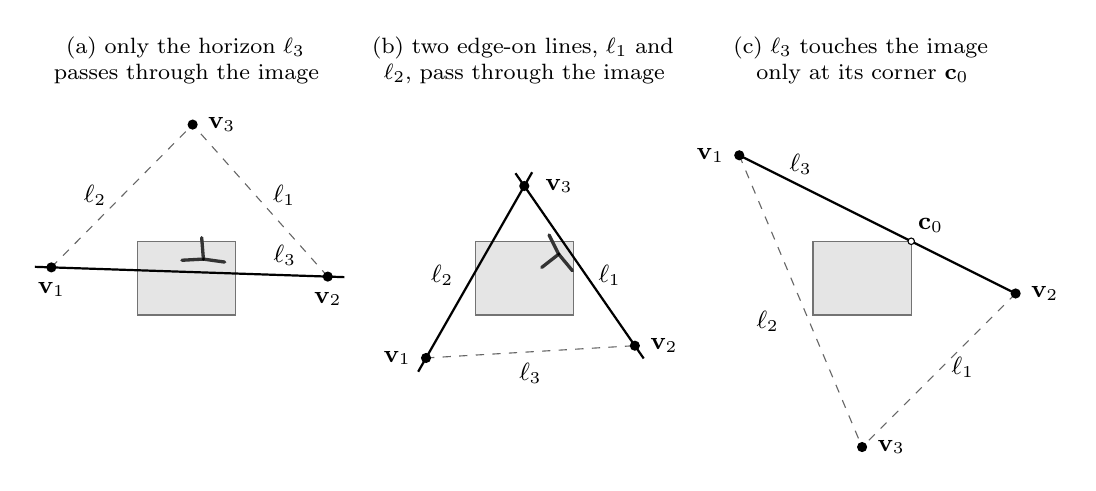
\begin{tikzpicture}[scale=0.39,font=\small]
\tikzset{img/.style={fill=black!10,draw=black!55},vp/.style={circle,fill,inner sep=1.3pt},
         pass/.style={thick},miss/.style={dashed,black!60},edge/.style={very thick,black!80,line cap=round},
         ttl/.style={font=\footnotesize,align=center,text width=3.8cm}}
% ---------------- (a) a nearly level camera: only the horizon passes through the image
\begin{scope}
  \draw[img] (-1.6,-1.2) rectangle (1.6,1.2);
  \coordinate (a1) at (-4.4,0.35); \coordinate (a2) at (4.6,0.05); \coordinate (a3) at (0.2,5.0);
  \draw[pass] ($(a1)!-0.06!(a2)$) -- ($(a2)!-0.06!(a1)$);
  \draw[miss] (a1) -- (a3); \draw[miss] (a2) -- (a3);
  \node[vp,label=below:{$\vv_1$}] at (a1) {}; \node[vp,label=below:{$\vv_2$}] at (a2) {}; \node[vp,label=right:{$\vv_3$}] at (a3) {};
  \node[above] at (3.2,0.1) {$\ell_3$}; \node[left] at (-2.3,2.7) {$\ell_2$}; \node[right] at (2.5,2.7) {$\ell_1$};
  \coordinate (c) at (0.55,0.62);
  \draw[edge] (c) -- ($(c)!0.7cm!(a1)$); \draw[edge] (c) -- ($(c)!0.7cm!(a2)$); \draw[edge] (c) -- ($(c)!0.7cm!(a3)$);
  \fill (c) circle (1.6pt);
  \node[ttl,anchor=south] at (0,6.0) {(a) only the horizon $\ell_3$ passes through the image};
\end{scope}
% ---------------- (b) an oblique view: two edge-on lines pass through the image
\begin{scope}[shift={(11,0)}]
  \draw[img] (-1.6,-1.2) rectangle (1.6,1.2);
  \coordinate (b1) at (-3.2,-2.6); \coordinate (b2) at (3.6,-2.2); \coordinate (b3) at (0.0,3.0);
  \draw[miss] (b1) -- (b2);
  \draw[pass] ($(b1)!-0.08!(b3)$) -- ($(b3)!-0.08!(b1)$); \draw[pass] ($(b2)!-0.08!(b3)$) -- ($(b3)!-0.08!(b2)$);
  \node[vp,label=left:{$\vv_1$}] at (b1) {}; \node[vp,label=right:{$\vv_2$}] at (b2) {}; \node[vp,label={[xshift=2pt]right:{$\vv_3$}}] at (b3) {};
  \node[below] at (0.2,-2.45) {$\ell_3$}; \node[left] at (-2.0,0.1) {$\ell_2$}; \node[right] at (2.1,0.1) {$\ell_1$};
  \coordinate (c) at (1.12,0.78);
  \draw[edge] (c) -- ($(c)!0.7cm!(b1)$); \draw[edge] (c) -- ($(c)!0.7cm!(b2)$); \draw[edge] (c) -- ($(c)!0.7cm!(b3)$);
  \fill (c) circle (1.6pt);
  \node[ttl,anchor=south] at (0,6.0) {(b) two edge-on lines, $\ell_1$ and $\ell_2$, pass through the image};
\end{scope}
% ---------------- (c) the touching case
\begin{scope}[shift={(22,0)}]
  \draw[img] (-1.6,-1.2) rectangle (1.6,1.2);
  \coordinate (c1) at (-4.0,4.0); \coordinate (c2) at (5.0,-0.5); \coordinate (c3) at (0.0,-5.5);
  \draw[pass] (c1) -- (c2); \draw[miss] (c1) -- (c3); \draw[miss] (c2) -- (c3);
  \draw[fill=white] (1.6,1.2) circle (3pt);
  \node[vp,label=left:{$\vv_1$}] at (c1) {}; \node[vp,label=right:{$\vv_2$}] at (c2) {}; \node[vp,label=right:{$\vv_3$}] at (c3) {};
  \node[above right=-1pt] at (1.6,1.25) {$\vc_0$};
  \node[above] at (-2.0,3.05) {$\ell_3$}; \node[left] at (-2.4,-1.4) {$\ell_2$}; \node[right] at (2.6,-2.9) {$\ell_1$};
  \node[ttl,anchor=south] at (0,6.0) {(c) $\ell_3$ touches the image only at its corner $\vc_0$};
\end{scope}
\end{tikzpicture}
\caption{The three vanishing points of a rectilinear structure, the edge-on lines that join them, and the image (gray). The edge-on line $\ell_k$ of axis $k$ passes through the other two vanishing points; solid lines meet the image and dashed lines miss it. Near a line that passes through the image, a junction's two edges toward that line's vanishing points nearly line up, the face they span being seen edge-on, as drawn in (a) and (b); such junctions reject every camera under which the opposite vanishing point is not perpendicular to the other two (\cref{thm:converse}). (a) A nearly level camera, for which few junctions are bounded above. (b) An oblique view, which forces all three perpendicularities. (c) The touching case, which forces the single linear condition \eqref{eq:touch}}
\label{fig:vlines}
\end{figure*}

\begin{theorem}[Which cameras one frame's junctions reject]\label{thm:converse}
Let the image $\mathcal I$ be a closed convex polygon with nonempty interior and no vanishing point on its boundary, and consider the junctions of one Manhattan frame with vertices in $\mathcal I$, off the vanishing lines. For an axis $k$, let $i$ and $j$ be the other two.
\begin{enumerate}
\item If $\vc_0\in\ell_k\cap\mathcal I$ is not a vanishing point, every positive-definite $\omega^{*}$ that violates
\begin{equation}
\zeta_j(\vc_0)\,N_{ik}=\zeta_i(\vc_0)\,N_{jk}
\label{eq:touch}
\end{equation}
is rejected by every junction whose vertex is close enough to $\vc_0$, how close depending on $\omega^{*}$. Hence, if $\ell_k$ meets $\mathcal I$ in a segment, every camera with $(N_{ik},N_{jk})\neq0$ is rejected by some junction; if it meets $\mathcal I$ only at a corner $\vc_0$, every camera that violates \eqref{eq:touch} is.
\item There is a constant $C$, depending only on the frame and on $\mathcal I$, such that every $\omega^{*}$ that satisfies the conditions of part (1) and has $\max_{b\neq c}|N_{bc}|<\min_aN_{aa}/C$ passes every junction.
\item If two vanishing lines meet $\mathcal I$ in segments, the cameras that pass every junction are exactly those that make the three vanishing points mutually orthogonal,
\begin{equation}
\omega^{*}=\sum_{k=1}^{3}\theta_k\,\vv_k\vv_k^{\top},\qquad \theta_k>0 .
\label{eq:vpfamily}
\end{equation}
\end{enumerate}
\end{theorem}
\begin{proof}
(1) Let $\vc_0\in\ell_k\cap \mathcal I$ not be a vanishing point, so that $\zeta_i,\zeta_j\neq0$ there, and let the vertex tend to $\vc_0$ from the interior of $\mathcal I$, off the vanishing lines, so that $\zeta_k\to0$. Put $B=(\zeta_i/\zeta_j)N_{jk}-N_{ik}$. By \eqref{eq:nuframe},
\[
\begin{aligned}
\nu_i&=N_{ii}-\frac{\zeta_i}{\zeta_j}N_{ij}+\frac{\zeta_i}{\zeta_k}\,B,\\
\nu_j&=N_{jj}-\frac{\zeta_j}{\zeta_i}N_{ij}-\frac{\zeta_j^2}{\zeta_i\zeta_k}\,B .
\end{aligned}
\]
The terms without $B$ stay bounded, and the two coefficients of $B$ are unbounded with opposite signs, whichever side of $\ell_k$ the vertex is on. Unless $B\to0$, one of $\nu_i$, $\nu_j$ is therefore negative at junctions arbitrarily near $\vc_0$, and by \cref{lem:frame} those are not admitted. So $B(\vc_0)=0$, which is \eqref{eq:touch}. Along a segment the ratio $\zeta_i/\zeta_j$ is a projective coordinate and is not constant, so \eqref{eq:touch} at two of its points gives $N_{ik}=N_{jk}=0$. A line meets a convex polygon in a single point only at a corner of the polygon, which by hypothesis is not a vanishing point.

(2) By \cref{lem:frame}, a camera passes every junction exactly when every $\nu_a$ of \eqref{eq:nuframe} is positive throughout $\mathcal I$. Suppose first that a vanishing point lies in $\mathcal I$. It is interior, the two vanishing lines through it meet $\mathcal I$ in segments, and the conditions of part (1) make $N$ diagonal, so that $\nu_a=N_{aa}>0$. Otherwise, in the expression \eqref{eq:nuframe} for $\nu_a$ the terms that are singular near $\ell_p\cap \mathcal I$ combine, exactly as above, into a bounded multiple of $B/\zeta_p$, with $B$ the quantity belonging to the line $\ell_p$, the other two coordinates being bounded away from zero there. If $\ell_p$ meets $\mathcal I$ in a segment, $B$ vanishes identically. If it meets $\mathcal I$ at a corner $\vc_0$, then, in the notation of part (1) with $p$ in place of $k$, $B=(\zeta_i/\zeta_j-t_0)N_{jp}$, with $t_0$ the value of the ratio at $\vc_0$; and $\mathcal I$ lies in a wedge at $\vc_0$ whose sides make positive angles with the line, so that the distance from $\vc_0$ is at most a constant times $|\zeta_p|$ on $\mathcal I$ and $B/\zeta_p$ is bounded by a constant times $|N_{jp}|$. Hence there is a constant $C$, depending only on the frame and on $\mathcal I$, with $|\nu_a-N_{aa}|\le C\max_{b\neq c}|N_{bc}|$ throughout $\mathcal I$, so that $\nu_a\ge N_{aa}-C\max_{b\neq c}|N_{bc}|>0$ whenever $\max_{b\neq c}|N_{bc}|<\min_aN_{aa}/C$.

(3) Two segments annihilate all three off-diagonal entries, so $N$ is diagonal, with positive entries because it is positive-definite, and $\omega^{*}=VNV^{\top}$ is \eqref{eq:vpfamily} with $\theta_k=N_{kk}$. Conversely, for diagonal $N$, \eqref{eq:nuframe} gives $\nu_a=N_{aa}>0$ at every junction.
\end{proof}

In part (1), $(N_{ik},N_{jk})\neq0$ says that $\vv_k$ is not orthogonal to the other two vanishing points under the camera. A vanishing line that misses $\mathcal I$ rejects no camera on this account, although the inequalities \eqref{eq:nuframe}, which a camera must satisfy throughout $\mathcal I$ to pass every junction (\cref{lem:frame}), still bound it. If no edge-on line touches $\mathcal I$, the constant of part (2) can be taken as $C=\sup_{\vc\in\mathcal I}\max_a\sum|\kappa_{a,bc}|$, the sum running over the off-diagonal entries $N_{bc}$ that part (1) does not force to vanish, with $\kappa_{a,bc}$ their coefficients in \eqref{eq:nuframe}; each coefficient is bounded on $\mathcal I$, because its denominator vanishes only on an edge-on line that misses $\mathcal I$. Near the true camera, the cameras that pass every junction therefore form a family whose dimension is that of the linear space cut out by the conditions of part (1). A camera that violates \eqref{eq:touch} only slightly is rejected only by junctions close to $\ell_k$. The theorem guarantees that such junctions exist; \OR{} (Sect.~S9) estimates how many junctions placed at random it takes to meet one. The constant $C$ of part (2) grows as a vanishing line that misses $\mathcal I$, or a vanishing point outside $\mathcal I$, comes close to $\mathcal I$, and as the angle of a touching wedge shrinks. The global admitted set is not characterized in general, and the number of conditions forced is the rank of the system of part (1), not the sum of per-line counts.

In the commonest case, the admitted set can be described globally rather than only near the true camera.

\begin{proposition}[One edge-on line through the image]\label{prop:oneline}
Under the hypotheses of \cref{thm:converse}, let $\ell_k$ meet $\mathcal I$ in a segment and let $\ell_i$ and $\ell_j$ miss $\mathcal I$. Let $r_-\le r_+$ be the extremes over $\mathcal I$ of $r=\zeta_i/\zeta_j$, which have one sign and are attained at corners of $\mathcal I$, and let $u^{\star}$ be the extreme over $\mathcal I$ of $u=\zeta_k^2/(\zeta_i\zeta_j)$, which has the sign of $r$. Up to its boundary, the set of positive-definite $\omega^{*}=VNV^{\top}$ that admit every junction of the frame with vertex in $\mathcal I$ is
\begin{equation}
\begin{aligned}
&N_{ik}=N_{jk}=0,\qquad N_{kk}+u^{\star}N_{ij}>0,\\
&N_{ii}>r_{\pm}N_{ij},\qquad N_{jj}>N_{ij}/r_{\pm},
\end{aligned}
\label{eq:oneline}
\end{equation}
five linear inequalities on the one free off-diagonal entry and the diagonal.
\end{proposition}
\begin{proof}
By \cref{thm:converse}(1) every admitted camera has $N_{ik}=N_{jk}=0$, and then \eqref{eq:nuframe} reduces to $\nu_i=N_{ii}-rN_{ij}$, $\nu_j=N_{jj}-N_{ij}/r$ and $\nu_k=N_{kk}+uN_{ij}$. Since $\ell_i$ and $\ell_j$ miss $\mathcal I$, $\zeta_i$ and $\zeta_j$ do not vanish on $\mathcal I$, so $r$ and $u$ have constant signs there, $r$ is a ratio of two affine functions and attains its extremes at corners of the convex polygon $\mathcal I$, and $u$ ranges from values arbitrarily close to $0$, near $\ell_k$, to $u^{\star}$. For fixed $N$, $\nu_i$ is affine in $r$, $\nu_j$ in $1/r$ and $\nu_k$ in $u$, so each is positive over its range exactly when it is positive at the ends of the range, up to the boundary; at the end $u\to0$ the condition is $N_{kk}>0$, which positive-definiteness already gives.
\end{proof}

For the camera of \OR{} (Sect.~S11), tilted by $4^\circ$, \eqref{eq:oneline} with unit diagonal gives the free entry the interval $(-0.882,\,0.286)$, which the numerical interval $[-0.88,\,0.28]$ found there matches to its grid step. For the same camera the constant of \cref{thm:converse}(2) is $C=3.50$, and its sufficient condition $|N_{12}|<1/C=0.286$ reproduces the upper end of this interval exactly. With the frame oriented differently, a dense sample of $1.5$ million junctions confirms both ends of the formula to within its grid step of $0.005$.

\begin{proposition}[One frame cannot calibrate a general camera]\label{prop:oneframe}
Every camera of the family \eqref{eq:vpfamily} admits every junction of the frame, wherever its vertex lies. The family has three parameters, two once $\omega^{*}$ is normalized, so the junctions of one frame, however many, never determine a general camera.
\end{proposition}
\begin{proof}
For diagonal $N$, \eqref{eq:nuframe} gives $\nu_a=N_{aa}>0$ for every $\boldsymbol\zeta$.
\end{proof}

The family \eqref{eq:vpfamily} is the classical one: the cameras under which the three vanishing points of the frame are mutually orthogonal \citep{hartley2004}. The reason is that every line of direction $k$, in every junction of the frame, passes through the same vanishing point $\vv_k$, so any number of junctions encodes only the frame's vanishing points. \Cref{thm:converse} determines how much of that information they retain, and the answer depends on the image. 

By \cref{thm:converse}, each vanishing line contributes two conditions when it meets the image in a segment, one when it touches the image only at a corner, and none when it misses the image. Lines in general position either pass through the image or miss it, so the number of conditions one frame forces is $0$, $2$ or $3$: three when at least two lines are in view, and two when one is, as when only the horizon passes through the image. The touching case is exceptional but real; \OR{} (Sect.~S11) gives an example. One frame can therefore determine a camera only if the camera model has no more parameters than the frame forces conditions. A single focal length needs one, and \cref{thm:identframe} says when one frame supplies it; a general camera needs five, which one frame never supplies.

\subsection{Several frames}\label{sec:frames}

One frame never determines a general camera (\cref{prop:oneframe}). Several frames can, provided their axes point in enough different directions, and the next theorem says exactly when.

Let Manhattan frames $R_1,\dots,R_n$ be seen by one camera $K$, possibly in different images, and write a candidate camera as $\omega^{*}=K\Xi K^{\top}$, so that $\Xi=I$ is the true one. An axis is a direction without regard to sign; call it \emph{visible} if its vanishing line meets the image area $\mathcal I$ in a segment, and \emph{touching} if the line meets $\mathcal I$ in a single point $\vc_0$, whose ray is $\vr_0=K^{-1}\vc_0$.

\begin{theorem}[Several frames]\label{thm:frames}
Consider all the junctions of the frames with vertices in an image area $\mathcal I$ that satisfies the hypotheses of \cref{thm:converse} for every frame.
\begin{enumerate}
\item Every positive-definite $\omega^{*}=K\Xi K^{\top}$ that admits all these junctions has each visible axis $\vd$ as an eigenvector of $\Xi$ and, for each touching axis $\vd$, $\Xi\vd$ in the plane spanned by $\vd$ and $\vr_0$; conversely, every $\Xi$ near $I$ that satisfies these conditions is admitted. If two axes of each frame are visible, the admitted cameras are exactly those with $\Xi$ positive-definite and diagonal in each frame.
\item The junctions determine $\omega^{*}$, up to scale, if and only if the only symmetric $\Xi$ that satisfy the conditions of (1) are the multiples of $I$. If no axis is touching, this holds if and only if the visible axes do not all lie in the union of a plane through the origin and the line normal to it.
\end{enumerate}
\end{theorem}
\begin{proof}
For a frame $R$ scale the vanishing points as $V=KR$. The matrix of \cref{lem:frame} is then $N=R^{\top}\Xi R$, so that $N_{ab}=\vd_a^{\top}\Xi\vd_b$, and at a point with ray $\vr$ the coordinates are $\zeta_a=\vd_a\cdot\vr$. By \cref{thm:converse}(1) a visible axis $\vd_k$ forces $N_{ik}=N_{jk}=0$, that is, $\Xi\vd_k$ is perpendicular to $\vd_i$ and $\vd_j$ and hence parallel to $\vd_k$. A touching axis forces \eqref{eq:touch}, which reads $\vd_k^{\top}\Xi\,\mathbf w=0$ with $\mathbf w=\zeta_j(\vc_0)\,\vd_i-\zeta_i(\vc_0)\,\vd_j$. Since $\zeta_k(\vc_0)=0$, $\vr_0=\zeta_i\vd_i+\zeta_j\vd_j$, so $\mathbf w$ is perpendicular to both $\vd_k$ and $\vr_0$; it is nonzero, because $\vc_0$ is not a vanishing point, and so it is a nonzero multiple of $\vd_k\times\vr_0$. The condition therefore says that $\Xi\vd_k$ lies in the plane spanned by $\vd_k$ and $\vr_0$. Conversely, \cref{thm:converse}(2) admits every $\Xi$ near $I$ that satisfies these conditions for one frame, uniformly over its junctions through the constant $C$, and so, the frames being finitely many, every $\Xi$ near $I$ that satisfies them for all. If two axes of each frame are visible, $N$ is diagonal by \cref{thm:converse}(3), which is the last statement of (1).

For (2), the conditions are linear in $\Xi$ and are satisfied by $I$. If their only solutions are the multiples of $I$, every admitted $\omega^{*}$ is a multiple of $KK^{\top}$, which is admitted. If they have a solution $\Xi_1$ that is not a multiple of $I$, they have $I+t\,\Xi_1$ for every $t$; it is positive-definite and admitted for $t$ near $0$ by (1), and it is not a multiple of $I$ when $t\neq0$. Suppose now that no axis is touching. A symmetric matrix that is not a multiple of $I$ has either three distinct eigenvalues, and then its eigenvectors are three mutually orthogonal lines, or exactly two equal, and then they are a plane and its normal; in either case they lie in the union of a plane and its normal. If the visible axes do not, the conditions therefore have only the multiples of $I$ as solutions. If they lie in a plane with normal $\mathbf n$, each of them is an eigenvector of $I+t\,\mathbf n\mathbf n^{\top}$.
\end{proof}

If the visible axes do lie in a plane and along its normal $\mathbf n$, the matrix $\mathbf n\mathbf n^{\top}$ satisfies the conditions of part (1), so the cameras $K(I+t\,\mathbf n\mathbf n^{\top})K^{\top}$ are admitted for all $t$ near $0$, by the proof of part (2). When every frame shows two of its vanishing lines, part (1) describes the admitted cameras globally, and the condition of part (2) becomes that no axis is common to all the frames. Indeed, an orthonormal triple contained in a plane and its normal must contain the normal, since the plane holds at most two orthonormal vectors, so every frame then has the normal as an axis. Conversely, if all the frames share an axis $\vd$, the matrices $I+t\,\vd\vd^{\top}$, $t>-1$, are positive-definite and diagonal in each frame. They are the only ones as soon as two of the frames have no other axis in common, because a symmetric form that is diagonal in two orthonormal bases of the plane $\vd^{\perp}$ sharing no direction is a multiple of the identity there.



At the other extreme, an image may show only its horizon, the vanishing line of the vertical. It then contributes a single visible axis, its vertical direction in camera coordinates.

\begin{corollary}[Images that show only their horizons]\label{cor:horizons}
Let three or more images taken with one camera each show only the horizon of their frame, passing through the image, and let no two of their vertical directions be perpendicular. Their junctions determine a general camera if and only if the vertical vanishing points of the images are not collinear. If the camera only pitches between them, the cameras $K(I+t\,\mathbf e_1\mathbf e_1^{\top})K^{\top}$, which differ from the true one only in the aspect ratio, are admitted for $t$ near $0$; if it only rolls, the cameras $K(I+t\,\mathbf e_3\mathbf e_3^{\top})K^{\top}$ are, a focal-length ambiguity.
\end{corollary}
\begin{proof}
The visible axes are the vertical directions $\mathbf g_m$. When no two are perpendicular, they lie in the union of a plane and its normal only if they lie in the plane, since one along the normal would be perpendicular to the rest; and directions are coplanar exactly when their vanishing points $K\mathbf g_m$ lie on one line, the vanishing line of their plane. \Cref{thm:frames}(2) gives the first statement. Pitching keeps every $\mathbf g_m$ perpendicular to $\mathbf e_1$, and rolling keeps it in the image plane, perpendicular to $\mathbf e_3$, so \cref{thm:frames}(2) gives the two families.
\end{proof}

At least three images are therefore needed, and the camera must do more than rotate about one axis between them.





A touching axis adds one condition where a visible one adds two. Applied to the cameras $\operatorname{diag}(f',f',1)$, these conditions reproduce \cref{thm:identframe}, including its exceptional point (\OR, Sect.~S11).

\subsection{The focal length: identifiability}\label{sec:identifiability}

For a camera whose only unknown is the focal length, \cref{lem:frame} can be solved explicitly, and the joint admissible set of one frame's junctions takes a closed form.

\begin{proposition}[The joint admissible set in closed form]\label{prop:gform}
Let $K=\operatorname{diag}(f,f,1)$, scale the vanishing points of a frame $R$ as $V=KR$, so that $\zeta_a=\vr\cdot\vd_a$ for the viewing ray $\vr=K^{-1}\vc$, and put $z_a=\vd_a\cdot\hat{\mathbf z}$, with $\hat{\mathbf z}$ the optical axis, and $w_a=z_a/\zeta_a$. For a candidate focal length $f'$, with $s=f'/f$, the quantities of \cref{lem:frame} at the junction with vertex $\boldsymbol\zeta$ are
\begin{equation}
\nu_a=s^2+(1-s^2)\,\gamma_a,\qquad \gamma_a=(z_a-\zeta_aw_p)(z_a-\zeta_aw_q).
\label{eq:gform}
\end{equation}
Consequently, for any set of junctions of the frame, writing $\Gamma^{+}$ and $\Gamma^{-}$ for the suprema of $\gamma_a$ and of $-\gamma_a$ over the junctions and over $a$,
\begin{equation}
\bigcap F=\Bigl\{f':\ \frac{\Gamma^{-}}{1+\Gamma^{-}}<\frac{f'^2}{f^2}<\frac{\Gamma^{+}}{\Gamma^{+}-1}\Bigr\}
\label{eq:capF}
\end{equation}
up to its endpoints, the upper bound being absent when $\Gamma^{+}\le1$. Here $\Gamma^{-}$ is positive as soon as one junction has no edge line through the principal point, by \cref{prop:bound}(1); when $\Gamma^{-}\le0$ there is no lower bound.
\end{proposition}
\begin{proof}
A focal length $f'$ lies in every $F$ exactly when $\omega^{*}=\operatorname{diag}(x,x,1)$, $x=f'^2$, admits every junction, and then
\[
\begin{aligned}
N&=R^{\top}K^{-1}\operatorname{diag}(x,x,1)K^{-\top}R\\
&=s^2I+(1-s^2)\,\mathbf z\mathbf z^{\top}.
\end{aligned}
\]
In \eqref{eq:nuframe}, $\nu_a$ is linear in $N$ and equals $1$ at $N=I$; at the rank-one $N=\mathbf z\mathbf z^{\top}$ its four terms factor as $(z_a-\zeta_az_p/\zeta_p)(z_a-\zeta_az_q/\zeta_q)=\gamma_a$, so $\nu_a=s^2+(1-s^2)\gamma_a$, which is \eqref{eq:gform}. At $s=1$ every $\nu_a$ equals $1$. For $s<1$, $\nu_a>0$ exactly when $-\gamma_a<s^2/(1-s^2)$, and this holds at every junction exactly when $\Gamma^{-}\le0$ or $s^2>\Gamma^{-}/(1+\Gamma^{-})$; for $s>1$, $\nu_a>0$ exactly when $\gamma_a<s^2/(s^2-1)$, which holds at every junction exactly when $\Gamma^{+}\le1$ or $s^2<\Gamma^{+}/(\Gamma^{+}-1)$.
\end{proof}

Each junction therefore bounds $f$ from below when some $\gamma_a$ is negative and from above when some $\gamma_a$ exceeds one, and the bounds approach $f$ as $\gamma$ becomes unbounded. Since $w_b$ is unbounded only where $\zeta_b\to0$ with $z_b\neq0$, the bounds can approach $f$ only near the edge-on line of an axis that is not parallel to the image plane; the question is what happens there. For a single junction, \eqref{eq:capF} gives the interval as an explicit function of the junction's position.

\begin{theorem}[Where a junction bounds the focal length]\label{thm:boundmap}
Let $K=\operatorname{diag}(f,f,1)$, let a frame have axes $\vd_a$, and for a vertex $\vc$ off the vanishing lines let $\vr=K^{-1}\vc$. For $\{a,p,q\}=\{1,2,3\}$,
\begin{equation}
\gamma_a=-\,\frac{\bigl(\vr\cdot(\hat{\mathbf z}\times\vd_p)\bigr)\bigl(\vr\cdot(\hat{\mathbf z}\times\vd_q)\bigr)}{(\vr\cdot\vd_p)(\vr\cdot\vd_q)},
\label{eq:boundmap}
\end{equation}
and the junction of the frame with vertex $\vc$ admits exactly the focal lengths $f'$ with $\Gamma^-/(1+\Gamma^-)<f'^2/f^2<\Gamma^+/(\Gamma^+-1)$, where $\Gamma^+=\max_a\gamma_a$ and $\Gamma^-=\max_a(-\gamma_a)$, the lower bound being absent when $\Gamma^-\le0$ and the upper when $\Gamma^+\le1$. It therefore bounds $f$ from above exactly when some $\gamma_a>1$, and from below by a positive value exactly when some $\gamma_a<0$. If the axes $p$ and $q$ are tilted, then
\begin{equation}
\gamma_a=1+\frac{z_pz_q\,(\vc-\vv_p)\cdot(\vc-\vv_q)}{f^2\,(\vr\cdot\vd_p)(\vr\cdot\vd_q)},
\label{eq:thales}
\end{equation}
with $\vc$ and the vanishing points in centered pixel coordinates. Hence $\{\gamma_a=1\}$ is the circle with diameter $\vv_p\vv_q$, on which the junction's edges toward $\vv_p$ and $\vv_q$ are perpendicular in the image, and the region $\gamma_a>1$ is bounded by this circle and the edge-on lines $\ell_p$ and $\ell_q$.
\end{theorem}
\begin{proof}
Write $R_b(\vr)=\vr\cdot(\hat{\mathbf z}\times\vd_b)$ and $\ell_b(\vr)=\vr\cdot\vd_b$; their zero sets are the line $R_b$ through the principal point and $\vv_b$ and the edge-on line $\ell_b$, and the claim is $\gamma_a=-R_pR_q/(\ell_p\ell_q)$. With $\zeta_b=\vr\cdot\vd_b$ and $z_b=\hat{\mathbf z}\cdot\vd_b$, \eqref{eq:gform} reads $\gamma_a=(z_a\zeta_p-\zeta_az_p)(z_a\zeta_q-\zeta_az_q)/(\zeta_p\zeta_q)$. By the expansion of the triple product, $z_a\zeta_p-\zeta_az_p=\vr\cdot\bigl(\hat{\mathbf z}\times(\vd_p\times\vd_a)\bigr)$, and $\vd_p\times\vd_a=-\varepsilon\vd_q$ with $\varepsilon=\det[\vd_1\,\vd_2\,\vd_3]=\pm1$; likewise $z_a\zeta_q-\zeta_az_q=\varepsilon\,\vr\cdot(\hat{\mathbf z}\times\vd_p)$. Since $\varepsilon^2=1$, this is \eqref{eq:boundmap}. One junction is a set of junctions, so \eqref{eq:capF} gives its interval, and the two bounds follow. For \eqref{eq:thales}, write $\vr=(\vc/f,1)$. The quadratic $Q=R_pR_q+\ell_p\ell_q$ in $\vc$ has no term in $xy$ and the coefficient $\bar\vd_p\cdot\bar\vd_q/f^2=-z_pz_q/f^2\neq0$ on $x^2$ and on $y^2$, so its zero set is a circle. The circle passes through $\vv_p$ and $\vv_q$, where $\vr$ is proportional to $\vd_p$ or $\vd_q$, and through $\vc^{\star}_p$, where $R_p$ meets $\ell_p$. There $R_p$, through $\vv_p$, meets $\ell_p$, through $\vv_q$, at a right angle, since $\ell_p$ has normal $\bar\vd_p$, so by Thales' theorem the circle is the one with diameter $\vv_p\vv_q$; it passes likewise through $\vc^{\star}_q$. The difference between $Q$ and $-(z_pz_q/f^2)(\vc-\vv_p)\cdot(\vc-\vv_q)$ has no quadratic terms and vanishes at $\vv_p$, $\vv_q$ and $\vc^{\star}_p$, which are not collinear, because $\vv_p$ is not on $\ell_p$, unless $\vc^{\star}_p=\vv_q$; so it is zero, by continuity in the frame also in that case, and \eqref{eq:thales} follows from \eqref{eq:boundmap}. The edge of the junction along $\vd_p$ lies on the line through $\vc$ and $\vv_p$, so on this circle the edges along $\vd_p$ and $\vd_q$ are perpendicular in the image. Finally, $\gamma_a-1$ changes sign only across this circle and the lines $\ell_p$ and $\ell_q$.\end{proof}

The circle of axis $a$ passes through the points $\vc^{\star}_p$ and $\vc^{\star}_q$ of the edge-on lines $\ell_p$ and $\ell_q$ nearest the principal point. The region in which a junction bounds the focal length from above is thus bounded by three circles, one for each axis, and by the edge-on lines (\cref{fig:boundmap}). On the circle of axis $a$, the junction's edges along the other two axes appear perpendicular: this is the raw right angle at which the threshold of that pair passes through infinity (\cref{thm:interval}). The circle is also the section by the image plane of the \emph{calibration sphere} with diameter $\vv_p\vv_q$, on which the center of projection lies because it sees $\vv_p$ and $\vv_q$ in perpendicular directions; in photogrammetry, this section is known as the locus of the isocenter \citep{grammatikopoulos2004}. The region hugs the edge-on lines of the tilted axes, where $\gamma$ is unbounded, and \cref{thm:identframe} states that it reaches $f$ from both sides when such a line passes through the image. On the York Urban images of \OR{} (Sect.~S12), the region covers a median $9.4\%$ of the image and a mean $12.3\%$; yet when the $181$ real junctions are replayed without noise, only $4$ of them, $2.2\%$, lie in it. Real corners avoid the neighborhoods of the edge-on lines, where two of their edges would look nearly collinear.

\begin{figure*}[t]
\centering
\includegraphics[width=0.92\linewidth]{figures/fig11_boundmap.pdf}
\caption{Where a junction bounds the focal length from above (\cref{thm:boundmap}). (a) A camera seen obliquely, the image outlined in black: junctions with vertices in the shaded region bound $f$ from above. Each axis contributes the circle with diameter between the other two vanishing points (dots), which passes through the points $\vc^{\star}$ (crosses), and the edge-on lines (dashed) complete the boundary. Of the two junctions drawn, the one far from every edge-on line has three distinct edges; the one marked ``on $\ell_1$'' lies on that line, where its two edges along the other axes fall on one image line, the face they span being seen edge-on. (b) A simulated nearly level camera, matched to York Urban ($640\times480$\,px, $f=675$\,px, a $3^\circ$ tilt): the region is a thin wedge along the horizon (dashed), covering $4\%$ of the image, and only $2$ of $15$ junctions at random positions (filled) lie in it, which is why upper bounds are rare for ordinary, nearly level cameras}
\label{fig:boundmap}
\end{figure*}

\begin{theorem}[Identifiability of the focal length from one frame]\label{thm:identframe}
Let the camera be $K=\operatorname{diag}(f,f,1)$ and the image a closed convex polygon with nonempty interior, such as a rectangle, with no vanishing point on its boundary; consider all the junctions of one Manhattan frame with vertices in the image and off its vanishing lines. Call an axis \emph{tilted} if it is not parallel to the image plane, and for a tilted axis $\vd_k$ let $\vc^{\star}_k$ be the point of its edge-on line $\ell_k$ nearest the principal point; if $\vd_k$ is the optical axis, that line is at infinity, never meets the image, and plays no part. Then $\bigcap F=\{f\}$ if and only if, for some tilted axis, $\ell_k$ meets the image at a point other than $\vc^{\star}_k$.
\end{theorem}
\begin{proof}
By \cref{prop:gform}, $\bigcap F=\{f\}$ exactly when $\gamma$ is unbounded above and below on the image. In the notation of the proof of \cref{thm:boundmap}, $\gamma_a=-R_pR_q/(\ell_p\ell_q)$, where the line $R_b$ through the principal point and $\vv_b$ is perpendicular to $\ell_b$ and meets it at $\vc^{\star}_b$. So $\gamma$ is bounded away from the edge-on lines, and the line $\ell_k$ of an untilted axis contributes nothing: it then passes through the principal point and coincides with $R_i$ and $R_j$, which cancel it.

Let $\ell_k$, with $z_k\neq0$, meet the image at a point $\vc_0$ that is not a vanishing point. The components with $\ell_k$ in their denominators are $\gamma_i=-(R_j/\ell_j)(R_k/\ell_k)$ and $\gamma_j=-(R_i/\ell_i)(R_k/\ell_k)$. On $\ell_k$, where $\vr=\zeta_i\vd_i+\zeta_j\vd_j$ and $\vd_i\times\vd_j=\varepsilon\vd_k$, we have $R_i=\varepsilon z_k\zeta_j$ and $R_j=-\varepsilon z_k\zeta_i$, so $(R_i/\ell_i)(R_j/\ell_j)=-z_k^2<0$ at $\vc_0$. As the vertex tends to $\vc_0$ from within the image, $R_k/\ell_k\to\pm\infty$ unless $R_k(\vc_0)=0$, that is, unless $\vc_0=\vc^{\star}_k$; then $\gamma_i$ and $\gamma_j$ diverge with opposite signs, whichever side of $\ell_k$ the vertex is on, and $\bigcap F=\{f\}$. A line that meets the image in more than one point meets it in a segment, which contains points other than $\vc^{\star}_k$ and the vanishing points; one that meets it in a single point meets it at a boundary point that is not a vanishing point. This proves sufficiency.

Conversely, if every edge-on line of a tilted axis that meets the image meets it only at its point $\vc^{\star}_k$, that point is a corner of the image, which lies in a wedge whose sides make positive angles with $\ell_k$. In the wedge, $|R_k|$, proportional to the distance from $R_k$, is at most a constant times $|\ell_k|$, so $R_k/\ell_k$ and hence $\gamma$ are bounded on the image, and $\bigcap F$ contains a neighborhood of $f$.
\end{proof}

A vanishing line need not pass through the image for its junctions to determine $f$: it suffices that the line reach the image, because a single junction near the line bounds $f$ from both sides at once, $\gamma_i$ and $\gamma_j$ having opposite signs. The exceptional point $\vc^{\star}_k$ is real, and \OR{} (Sect.~S10) shows its cost.

\begin{corollary}[A wide field of view suffices]\label{cor:wide}
Under the hypotheses of \cref{thm:identframe}, if no axis of the frame is parallel to the image plane and the image contains a cone of half-angle greater than $\arcsin(1/\sqrt3)\approx35.26^\circ$ about the optical axis, a circular field of view above $70.53^\circ$, then $\bigcap F=\{f\}$. The constant is sharp: for the frame seen down a cube diagonal, a circular field of view of at most $70.53^\circ$ does not determine $f$.
\end{corollary}
\begin{proof}
Since $\sum_a(\vd_a\cdot\hat{\mathbf z})^2=1$ for an orthonormal frame, some axis has $0<|z_a|\le1/\sqrt3$. Its edge-on line consists of the rays perpendicular to $\vd_a$, a plane that makes the angle $\arcsin|z_a|\le\arcsin(1/\sqrt3)$ with $\hat{\mathbf z}$. The line therefore meets the open cone, and so the interior of the image, in a segment, which contains points other than $\vc^{\star}_a$; \cref{thm:identframe} applies. For the cube diagonal every axis has $|z_a|=1/\sqrt3$, so each edge-on line keeps an angle of exactly $\arcsin(1/\sqrt3)$ from the optical axis; a circular image of at most that half-angle meets each line at most at its point $\vc^{\star}_a$, and \cref{thm:identframe} shows that $f$ is then not determined.
\end{proof}

The restriction to tilted axes matters in practice, because the commonest camera pose is nearly level. For a level camera, the vertical axis is parallel to the image plane and its edge-on line is the horizon, so $w_k=0$ and the horizon contributes nothing to $\gamma$. Concretely, if $u$ is the abscissa of the junction, the thresholds of the two pairs containing the vertical edge are $-u$ times the abscissae of the two horizontal vanishing points, independent of the junction's distance from the horizon. No junction near the horizon is therefore bounded above through its vertical edge. The horizontal axes of a level camera are tilted, however, and the edge-on line of each is the vertical image line through the other horizontal vanishing point. If neither horizontal vanishing point lies within the horizontal extent of the image, these lines miss it and upper bounds are rare; if one does, as in corridor or street views, its line passes through the image and \cref{thm:identframe} applies. Tilting the camera restores identifiability only gradually. Take $f=900$\,px and a $960$\,px square image, with vertices uniform over it and the horizontal vanishing points outside its horizontal extent, so that only the horizon is in view. The share of junctions bounded above is then $0.4\%$, $1.8\%$, $4.4\%$, $10.8\%$ and $22.2\%$ at tilts of $0.5^\circ$, $2^\circ$, $5^\circ$, $12^\circ$ and $25^\circ$, against none for a level camera, for which the intersection of $40\,000$ admissible sets is $[0.80f,\infty)$. \OR{} (Sect.~S12) finds the consequence in real images.

\paragraph{The mechanism at a single junction.} At the true camera, the interpretation-plane normal $\vn_m$ is parallel to $\vr\times\vd_m$, so for two orthogonal edges
\begin{equation}
\begin{aligned}
(\vr\times\vd_i)\cdot(\vr\times\vd_j)&=\|\vr\|^2(\vd_i\cdot\vd_j)-(\vr\cdot\vd_i)(\vr\cdot\vd_j)\\
&=-(\vr\cdot\vd_i)(\vr\cdot\vd_j).
\end{aligned}
\label{eq:edgeon}
\end{equation}
The pair form therefore vanishes at the true $f$ exactly when one of its two edges is \emph{perpendicular to the viewing ray}. Geometrically, $\vr\perp\vd_i$ places the ray in the face spanned by the other two edges, so that face is seen edge-on and those two edges project onto one image line: the configuration is the degeneracy of \cref{sec:sign}, approached rather than reached. The condition $\vr\perp\vd_i$ is the vanishing line $\ell_i$ of \cref{sec:oneframe} seen from a single junction: as the vertex approaches $\ell_i$, the thresholds of the two pairs that contain edge $i$ both tend to $f$, one from each side. The junctions that pin $f$ most tightly are therefore those that see a face nearly edge-on, which are also those closest to the degeneracy of two edges sharing an image line. 

\subsection{Focal length and principal point}\label{sec:fpp}

\Cref{thm:identframe} assumes the principal point known. When it is unknown as well, \cref{thm:frames}(1) still applies, and its conditions can be solved completely for a camera with square pixels and zero skew. For an axis $\vd$, write $\bar{\vd}\in\mathbb R^2$ for its first two coordinates, its direction in the image plane, and $z=\vd\cdot\hat{\mathbf z}$, as in \cref{prop:gform}; the axis is tilted when $z\neq0$.

\begin{theorem}[Focal length and principal point]\label{thm:fpp}
Let the camera have square pixels and zero skew, with its focal length and principal point unknown, and let the frames and visible axes be as in \cref{thm:frames}. The junctions determine the focal length and the principal point unless
\begin{enumerate}
\item no visible axis is tilted; or
\item the visible tilted axes are a single axis, or two perpendicular axes, lying in a plane $\Theta$ that contains the optical axis, and every other visible axis is normal to $\Theta$.
\end{enumerate}
If no axis is touching, then in case (1) the focal length is not determined, and in case (2) the admitted cameras near the true one form a one-parameter family, in which the principal point moves along the image of $\Theta$, the line through the principal point with direction $\bar{\vd}$, for any tilted axis $\vd$.
\end{theorem}
\begin{proof}
Write a candidate camera as $K'=KT$ with
\[
T=\begin{pmatrix} sI & \mathbf p\\ \mathbf 0^{\top} & 1\end{pmatrix},\qquad
\Xi=TT^{\top}=\begin{pmatrix} s^2I+\mathbf p\mathbf p^{\top} & \mathbf p\\ \mathbf p^{\top} & 1\end{pmatrix},
\]
where $s>0$ is the ratio of the focal lengths and $\mathbf p\in\mathbb R^2$ the displacement of the principal point divided by $f$. By \cref{thm:frames}(1) each visible axis $\vd$ satisfies $\Xi\vd=\lambda\vd$ with $\lambda>0$, that is,
\[
s^2\bar{\vd}+(\mathbf p\cdot\bar{\vd}+z)\,\mathbf p=\lambda\bar{\vd},\qquad \mathbf p\cdot\bar{\vd}+z=\lambda z .
\]
A visible axis is not the optical axis, whose vanishing line is at infinity, so $\bar{\vd}\neq0$. If $z=0$, the second equation gives $\mathbf p\cdot\bar{\vd}=0$, and the first then holds with $\lambda=s^2$. If $z\neq0$, substituting the second equation into the first gives $\lambda z\,\mathbf p=(\lambda-s^2)\,\bar{\vd}$, so $\mathbf p=m\bar{\vd}$ for some $m$, and then
\begin{equation}
\lambda=1+m\,\|\bar{\vd}\|^2/z,\qquad s^2=\lambda\,(1-mz).
\label{eq:fppaxis}
\end{equation}

Suppose some visible axis is tilted and case (2) does not hold. If two tilted axes have directions $\bar{\vd}$ that are not parallel, $\mathbf p=0$. Otherwise these directions are all multiples of one unit vector $\mathbf u$, the tilted axes lie in the plane $\Theta$ spanned by $(\mathbf u,0)$ and $\hat{\mathbf z}$, and $\mathbf p=h\mathbf u$. An untilted visible axis $\mathbf e$ with $\bar{\mathbf e}\cdot\mathbf u\neq0$ then gives $h=0$. If there is none, every untilted visible axis is normal to $\Theta$, and since case (2) does not hold, $\Theta$ contains two visible tilted axes that are neither equal nor perpendicular. Write them as $\vd_a=(c_a\mathbf u,z_a)$ with $c_a^2+z_a^2=1$, $a=1,2$, so that $m_a=h/c_a$. Then \eqref{eq:fppaxis} becomes
\[
s^2=1+\tau_ah-h^2,\qquad \tau_a=\frac{c_a}{z_a}-\frac{z_a}{c_a}=2\cot2\theta_a ,
\]
where $c_a=\cos\theta_a$ and $z_a=\sin\theta_a$. Now $\tau_1=\tau_2$ only if $\theta_1-\theta_2$ is a multiple of $\pi/2$, that is, only if the axes are equal or perpendicular, so $h=0$. In every case therefore $\mathbf p=0$; for a tilted axis $\lambda=1$, and the first equation gives $s=1$. The only camera that satisfies the conditions is the true one, and it is admitted.

Suppose finally that no axis is touching. In case (1) every visible axis has $z=0$, and $\mathbf p=0$ with any $s$ satisfies the conditions; by \cref{thm:frames}(1) the cameras with $s$ near $1$ are admitted, so the focal length is not determined. In case (2) all the tilted axes have the same $\tau_a=\tau$, for a single axis trivially and for two perpendicular ones by the remark above. Then $\mathbf p=h\mathbf u$ with $s^2=1+\tau h-h^2$ satisfies the conditions of every tilted axis, and of every untilted one, which is normal to $\Theta$ so that $\bar{\mathbf e}\cdot\mathbf u=0$; by \cref{thm:frames}(1) these cameras are admitted for $h$ near $0$.
\end{proof}

The exceptional configurations are classical. One frame with all three vanishing lines in view determines the camera unless one of its axes is parallel to the image plane, which is case (2), the failure of the orthocenter construction when a vanishing point is at infinity. A single image from a tilted camera showing only its horizon is also case (2): the principal point can slide along the line joining it to the vertical vanishing point; for a level camera the same image is case (1). 

\OR{} (Sect.~S5) gives the case of two images that show only their horizons. A touching axis adds one condition, which may remove the family of case (2); for the focal length alone, this is the statement of \cref{thm:identframe} that a vanishing line touching the image away from $\vc^{\star}_k$ determines $f$. 



\subsection{The convex program}\label{sec:program}

\Cref{thm:convex} turns calibration from junctions into a concrete convex program, because each junction's sign pattern is read from the junction alone, so the constraints can be written down without knowing $K$.

For a camera with known principal point and zero skew, $\omega^{*}=\operatorname{diag}(X,Y,1)$ and positive-definiteness reduces to $X,Y>0$, so the cameras consistent with $M$ junctions form the feasible set of a linear program, whose extent in $X$ and in $Y$ is again a linear program. For the full camera, with skew and principal point free, positive-definiteness is a matrix inequality, which we impose with cutting planes; this requires nothing beyond a linear-programming solver. From noiseless junctions of independent frames, every parameter is recovered to within about one pixel (\OR, Sect.~S11). From the junctions of a single frame, by \cref{prop:oneframe}, the program cannot close on a general camera; \OR{} (Sect.~S12) applies a robust form of it to real junctions.

\paragraph{Procedure.} (i) For each junction, read the three rank-one generators and their sign pattern from the junction alone (\cref{thm:convex}); each condition $\nu_k>0$ is then a linear inequality in the entries of $\omega^{*}$. (ii) Normalize $\omega^{*}_{33}=1$ and solve the linear program, with any objective, in a bounded box. In practice the box comes from loose prior bounds, for instance focal lengths between a tenth and ten times the image width and a principal point inside the image; it need only contain the true camera. (iii) If the solution is not positive-definite, add the cut $\mathbf v^{\top}\omega^{*}\mathbf v\ge0$ for the eigenvector $\mathbf v$ of its most negative eigenvalue and solve again, until the smallest eigenvalue is nonnegative to tolerance. (iv) The extent of each entry of $\omega^{*}$ is the value of a further linear program over the final feasible set. (v) Under noise the strict feasible set empties as junctions accumulate; replace it by a depth-$\kappa$ consensus, or weight each junction by its miss probability, as in \OR{} (Sects.~S7 and S8).

\begin{proposition}[The convex program]\label{prop:program}
Let $M$ junctions be admitted by a camera $K_0$, and normalize $\omega^{*}_{33}=1$.
\begin{enumerate}
\item The set of $\omega^{*}$ that admit all $M$ junctions is convex: the intersection of the positive-definite cone with the $3M$ open half-spaces $\nu^{(m)}_k(\omega^{*})>0$ of \cref{thm:convex}, one for each image line of each junction.
\item Run the procedure with the closed constraints $\nu^{(m)}_k\ge0$ in a compact box containing $K_0K_0^{\top}$. Then every linear program is feasible, the iterates $\omega_t$ satisfy $\liminf_t\lambda_{\min}(\omega_t)\ge0$, and every accumulation point satisfies all the junction constraints and is positive semidefinite. In particular, for every $\tau>0$ the stopping rule $\lambda_{\min}(\omega_t)\ge-\tau$ is met after finitely many cuts.
\end{enumerate}
\end{proposition}
\begin{proof}
(1) By \cref{thm:convex}, a junction is admitted exactly when its three coefficients $\nu_k$, each linear in $\omega^{*}$, are positive.

(2) The matrix $K_0K_0^{\top}$ satisfies every junction constraint and every cut $\mathbf v^{\top}\omega^{*}\mathbf v\ge0$, so every linear program is feasible, and, the box being compact, it has a solution $\omega_t$. Let $\mathbf v_s$ be the unit eigenvector whose cut is added at step $s$, so that $\mathbf v_s^{\top}\omega_s\mathbf v_s=\lambda_{\min}(\omega_s)$. Every later iterate satisfies that cut, so for $t>s$
\[
\lambda_{\min}(\omega_s)=\mathbf v_s^{\top}(\omega_s-\omega_t)\mathbf v_s+\mathbf v_s^{\top}\omega_t\mathbf v_s\ge-\|\omega_s-\omega_t\| .
\]
If $\omega_{t_m}\to\bar\omega$ along a subsequence, taking $s=t_m$ and $t=t_{m+1}$ gives $\lambda_{\min}(\omega_{t_m})\ge-\|\omega_{t_m}-\omega_{t_{m+1}}\|\to0$, so $\lambda_{\min}(\bar\omega)\ge0$ by continuity; and $\bar\omega$ satisfies the junction constraints, which hold at every iterate and are closed. Finally, if $\lambda_{\min}(\omega_t)<-\tau$ for infinitely many $t$, these iterates have, by compactness, a convergent subsequence whose limit has $\lambda_{\min}\le-\tau<0$, a contradiction. Hence $\liminf_t\lambda_{\min}(\omega_t)\ge0$, and for every $\tau>0$ the stopping rule $\lambda_{\min}(\omega_t)\ge-\tau$ is met after finitely many cuts.
\end{proof}

\paragraph{Under noise.} The strict intersection of admissible sets loses coverage as junctions accumulate, because a single wrong interval suffices to exclude the truth. \OR{} (Sect.~S8) gives a depth-$\kappa$ consensus whose coverage follows a binomial prediction, and a log-plausibility built on the noise analysis of Sect.~S7. In simulation, its maximizer needs ten to twenty junctions to come within $10\%$ of $f$ at $\sigma=0.5$\,px, several images' worth at the $1.8$ full junctions per image of York Urban (\OR, Sect.~S12).

\section{Experiments}\label{sec:experiments}

We check \cref{thm:interval} in simulation and then test the predictions on real images. \OR{} (Sect.~S10) gives the full protocol, the checks of the noise model of Sect.~S7, the identifiability transition behind \cref{thm:identframe}, and the robustness of the bound to the protocol's idealizations, among them other noise levels, a tilted camera and a misplaced principal point; the dependence on edge length is analyzed in Sect.~S7, lens distortion in Sect.~S6, and further experiments are in Sect.~S13. Offsetting the assumed principal point by up to $20$\,px leaves the coverage of the true focal length at $94$ to $98\%$ at all three fields of view.

\subsection{The focal-length bound}\label{sec:e2}
Corners are sampled uniformly over orientations and over a $1000\times1000$\,px image, at fields of view of $40^\circ$, $60^\circ$ and $90^\circ$ ($f=1374$, $866$ and $500$\,px), and each edge is observed as a $150$\,px segment whose endpoints carry Gaussian noise of standard deviation $\sigma$ (\OR, Sect.~S10). Over $1000$ corners per field of view, with $\sigma=0.5$\,px and $150$\,px edges, the admissible set $F$ contained the true $f$ in 98\%, 97\% and 97\% of cases at $40^\circ$, $60^\circ$ and $90^\circ$, and it was a single interval in all $3000$ cases, as \cref{thm:interval} requires. It was unbounded above for 90\%, 81\% and 66\% of corners, and a check at $\sigma=0$ confirmed in $3000$ of $3000$ cases that unboundedness coincides with the raw image angles passing the orthographic fork-or-arrow rule, as \cref{prop:bound}(2) states.

The lower bound rises with distance from the center: the median of $\fmin/f$ is $0.08$, $0.15$ and $0.21$ in the inner third of the image and $0.29$, $0.41$ and $0.52$ in the outer third, at the three fields of view (\OR, Sect.~S10). An upper bound appears for 13\%, 25\% and 43\% of outer-third corners, at a median of $1.3$ to $1.4$ times $f$. The similarity law of \cref{cor:similar} accounts for most of the variation with position. Measured in units of $\rho$ at $\sigma=0$, the median of $\fmin/\rho$ stays within a factor of two across bins of distance from the center and fields of view, whereas $\fmin/f$ ranges over a factor of seven (\OR, Sect.~S10). The growth of the bound with radius is therefore mostly the factor $\rho$ of \cref{cor:similar}; the remainder reflects how the angles $\psi_i$ are distributed over junctions.

\subsection{Real images}\label{sec:realsummary}

On the $102$ images of the York Urban Database \citep{denis2008}, the admissible set contained the true focal length for $179$ of $181$ real junctions, and the certified sets of \cref{prop:certified} for all of them. Only two junctions bounded the focal length from above: real corners avoid the neighborhoods of the edge-on lines, so the bounds do not calibrate this nearly level camera. Calibration from three vanishing points does better where line families are available. \OR{} (Sect.~S12) gives the data, the junction extraction and every number.

\section{Conclusion}\label{sec:conclusion}

A right-angle corner constrains an uncalibrated camera through a single identity: three image lines through a point are the image of such a corner under a given camera exactly when a product of three forms, each linear in the dual image of the absolute conic, is negative. Everything in this paper follows from it. One junction admits a convex cone of cameras, the same at every junction up to a linear change of coordinates, and a closed-form interval when only the focal length is unknown. With the vertex position known, these bounds can be certified against any bounded error in the measured edge directions. When the corners belong to one rectilinear structure, their junctions reject, for each axis whose edge-on line passes through the image, exactly the cameras under which that axis's vanishing point is not orthogonal to the other two, and no other cameras near the truth: junctions carry at most the information of the vanishing points. For the focal length, a junction bounds it from above exactly inside circles whose diameters join pairs of vanishing points, and the corners of one structure determine it when the edge-on line of a tilted axis passes through the image. Since each junction's constraint is computed from the image alone, calibration from junctions is a convex feasibility problem.

The experiments agree with the single-junction results, and on real images they mark the limit of the approach. Real corners avoid the neighborhoods of the edge-on lines, so a nearly level camera with an ordinary field of view obtains a near-tight lower bound on its focal length rather than an estimate, and line families, where they exist, remain the better route. The experiments do not reach the cluttered, close-range regime that motivates the theory; whether cluttered interiors and automatic junction detection change this picture is the open empirical question, and \OR{} (Sect.~S12) discusses this and the other limitations of the evaluation. Several theoretical questions remain open as well. Radial distortion acts on each junction by an explicit transformation (\OR, Sect.~S6), which suggests estimating the distortion coefficient from junctions rather than treating it as a nuisance. The admitted cameras are described globally when one edge-on line passes through the image (\cref{prop:oneline}), but not in general. Nor is the trihedral with known non-right angles characterized.

\backmatter

\section*{Declarations}

\paragraph{Funding.} No funding was received for conducting this study.

\paragraph{Competing interests.} The author has no competing interests to declare that are relevant to the content of this article.

\paragraph{Ethics approval and consent.} Not applicable.

\paragraph{Data availability.} The York Urban Database \citep{denis2008} analyzed in this study is publicly available from its authors. No new image data were generated.

\paragraph{Code availability.} The code that verifies every identity symbolically and regenerates every number and figure in this paper is submitted with this manuscript as Online Resource 2 and will be released in a public GitHub repository, whose address will be given in the published version.

\paragraph{Author contributions.} The author is the sole author of this work, with the assistance described below.

\paragraph{Use of AI tools.} This work was carried out with substantial assistance from a large language model, Claude (Anthropic), in the versions available during 2026, including Claude Opus 5.5. The author posed the research question, chose the problems to pursue, decided what to prove, what to include and what to set aside, and directed every revision, including the responses to referee reports. Under that direction, the tool proposed and developed derivations and proofs, including those of the main theorems; wrote the symbolic verification code and the experiment and figure code; ran the experiments on data that the author obtained; drafted and revised the text; and located and checked references. Every algebraic identity in the paper is checked symbolically by the supplied code, every reported number is regenerated by it, and every cited reference was checked against its publisher or an authoritative index. The author checked every theorem and proof personally, reviewed all the results, and takes full responsibility for the content of the paper.

\bibliography{refs}

\end{document}
